\subsection{Methodologies}
\label{sec:lfd}
This section is dedicated to present and analyze various approaches for solving the LfD problem described in Section~\ref{sec:problem_formulation}. Specifically,  the proposed taxonomy is derived from studying different review papers~\cite{kaelbling1996reinforcement_survey,argall2009robot_learning_from_demonstration,hussein2017imitation_learning_survey,fang2019survey,zheng2021imitation_progress_taxonomies_opportunities,zare2024survey}. Figure~\ref{fig:il_taxonomy} provides a graphical representation of the proposed taxonomy. The methods are first categorized based on the type of demonstration, either \textit{State-Action} or \textit{State-only}, followed by an overview of the different methodologies. The proposed taxonomy highlights the learning algorithm and main components for each methodology.

This chapter is divided into the following sections. Section~\ref{sec:bc} reviews methods for the fully-supervised learning methodology known as \textit{Behavioral Cloning}. 
\newline Section~\ref{sec:irl} discusses methods under the umbrella of \textit{Inverse Reinforcement Learning}, which solve the inverse optimization problem by first learning the reward function and then using it to guide policy optimization following a reinforcement paradigm.
\newline Section~\ref{sec:gail} reviews methods leveraging the concept of \textit{Generative Adversarial Learning} to optimize policy parameters and learn demonstrated behaviors, classified as Generative Adversarial Imitation Learning methods.
\newline Finally, Section~\ref{sec:lfo} covers the most recent methodology, \textit{Learning from Observation}, characterized by optimizing the learner policy using state-only demonstrations.
\begin{figure}[tb]
    
    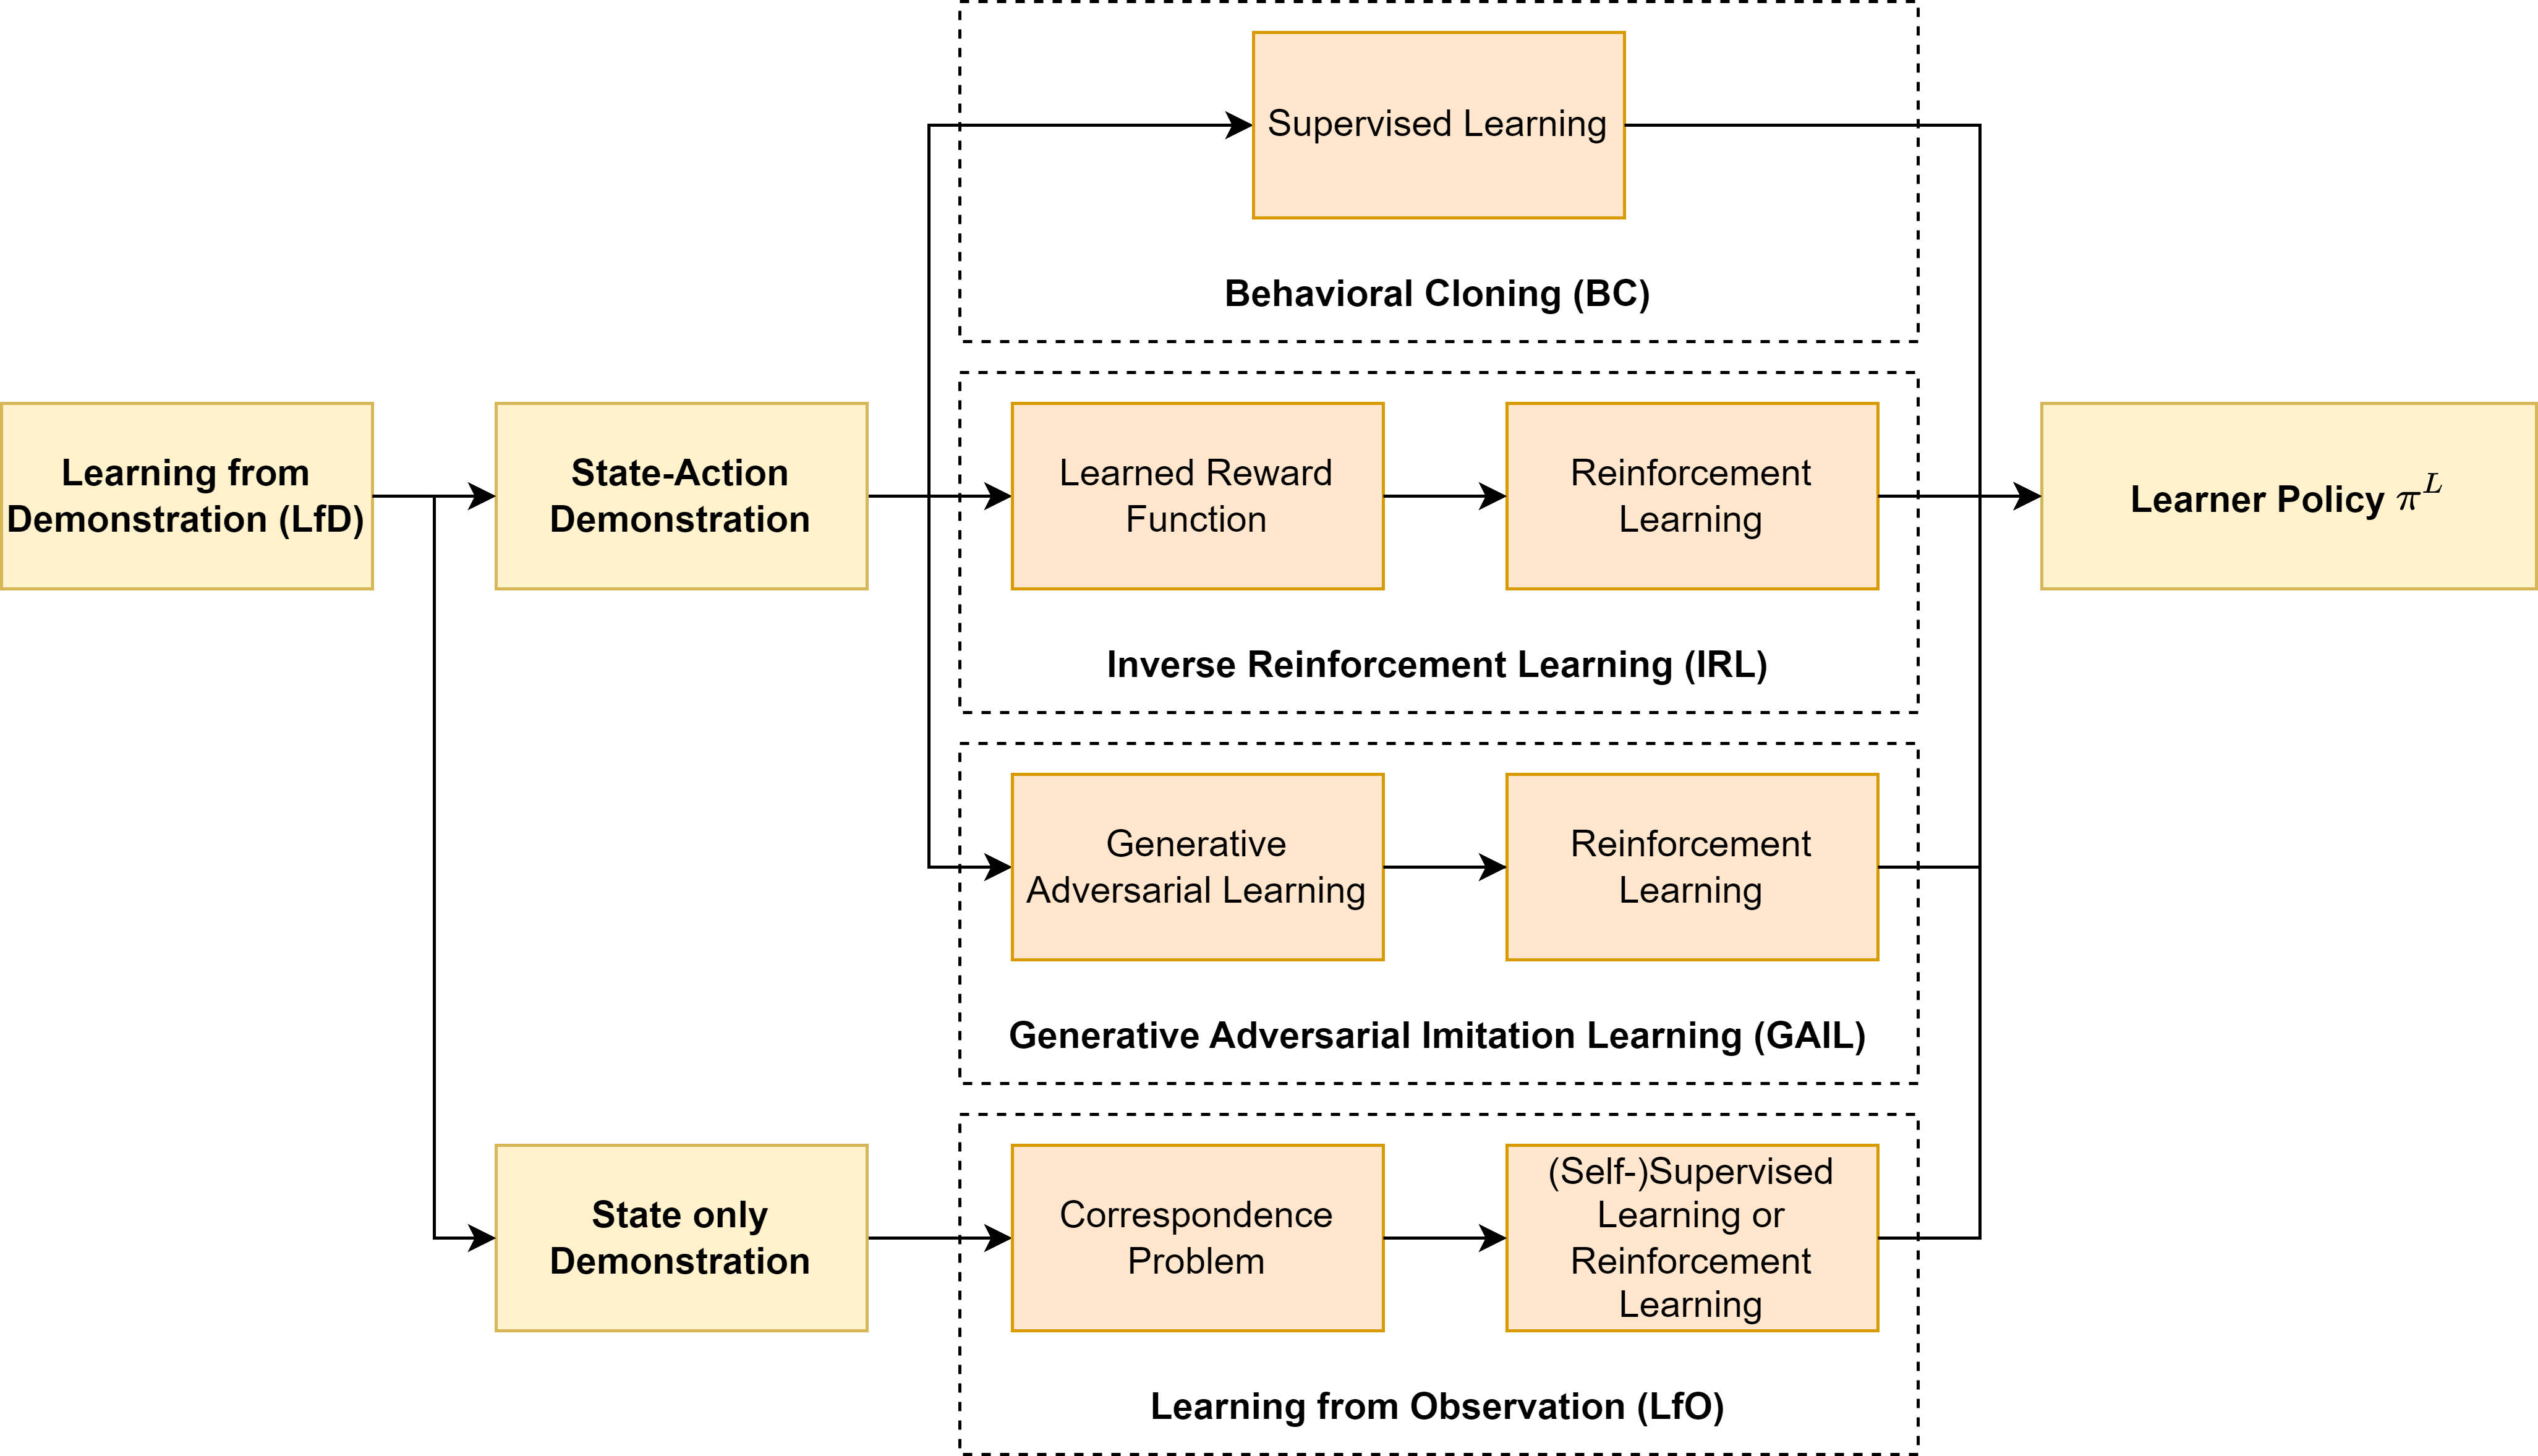
\includegraphics[width=\textwidth]{figures/images/il_taxonomy.png}
    \caption{Taxonomy of LfD methods, divided based on type of demonstration and the learning algorithm used to learn the learner policy $\pi^{L}$ }
    \label{fig:il_taxonomy}
    
\end{figure}


Each paragraph will present the research in the same way, i.e., the proposed works will be presented in a temporal order, highlighting the evolution of techniques and approaches over time.
It is important to note that with respect to the problem managed in this thesis, the most relevant and most related literature is the one presented in Section \ref{sec:bc}. However, for sake of clarity and completeness, all the other approaches will be described with their pros/cons, with some considerations with respect to the proposal of this thesis.


\subsubsection{Behavioral Cloning}
\label{sec:bc}
\begin{algorithm}[t]
\caption{Abstract Algorithm for BC methods}\label{alg:bc}
\begin{algorithmic}
\REQUIRE A set of expert demonstrations $\mathcal{D}^{E}$, a parameterized policy $\pi_{\theta}^{L}$
\ENSURE The optimal set of policy parameter $\theta^{*}$
\STATE Optimize $\mathcal{L}$ w.r.t.\ policy parameter $\theta$ using $\mathcal{D}^{E}$
\end{algorithmic}
\end{algorithm}
\textit{Behavioral Cloning} is one of the first approaches used to solve the LfD problem~\cite{pomerleau1988alvinn}. The high-level \textbf{supervised-learning} procedure followed by BC methods is outlined in Algorithm~\ref{alg:bc}. Generally, BC methods take as input the expert demonstration dataset $\mathcal{D}^{E}$ and a learner policy modeled as a parameterized function $\pi_{\theta}^{L}$. The parameters $\theta$ can be either the weights of a neural network~\cite{pomerleau1988alvinn} or the parameters of a dynamic system~\cite{ijspeert2002learning}. As a supervised approach, the goal is to find the optimal parameters $\theta^{*}$ that can replicate the \textbf{ground-truth behaviors} contained in the dataset $\mathcal{D}^{E}$. This is achieved by solving an optimization problem, which can generally be described by Formula~\ref{eq:bc_formula}.
\begin{equation}
 \label{eq:bc_formula}
 \theta^{*} = \underset{\theta}{argmin} \ \mathbb{E}_{(\boldsymbol{\tau}, c) \sim \mathcal{D}^{E}} \ [\mathcal{L}((\boldsymbol{\tau}, c), \ \pi^{L}_{\theta})]
\end{equation}


In the following section, different ways in which the general optimization problem described by Formula~\ref{eq:bc_formula} is formulated and solved will be discussed.

\paragraph*{Dynamical Movement Primitives}\mbox{}\\
% Dynamical Movement Primitives (DMPs), offer a robust framework for encoding and reproducing complex movements through differential equations and attractor dynamics.
The \textit{Dynamical-Movement Primitives} (DMPs) methods are among the first successful applications of the BC methodology to the LfD problem. Their success is attributed to their ease of implementation and efficiency in learning. DMPs do not require learning or estimating the system dynamics, nor do they require a reward function or interaction with the environment during the learning procedure, as they are supervised learning methods.

DMPs were first formalized in \cite{ijspeert2002learning}. They derive the policy directly in the trajectory space, allowing for explicit modeling of constraints such as smooth convergence toward the goal state. The core idea behind DMPs, as proposed in \cite{ijspeert2002learning,ijspeert2013dynamical}, is to model the trajectory as a \textbf{point-to-point attractor system}, described by the set of differential equations in Formula~\ref{eq:dmp}.
\begin{equation}
    \begin{matrix}
        \tau \dot{y} = \beta_{s}(\alpha_{s}(g-s)- y) + f(z) \\
        \\
         \tau \dot{s} = y\\
         \\
         \tau \dot{z} = -\alpha_{z} z, \ z(t) = z_{0} \ exp(-\frac{\alpha_{z}}{\tau} t)
        \end{matrix}
    \label{eq:dmp}
\end{equation}


Here, $\beta_{s}$, $\alpha_{s}$, and $\alpha_{z}$ are constants, $s$ is the system state, $z$ is the phase-variable function of time $t$, and $f$ is the forcing term that describes the trajectory's non-linear behavior. Generally, $f$ is a linear combination of basis functions $\psi_{i}(z)$ (e.g., Gaussian basis functions), such that $f(z(t)) = (g - s_{0}) \sum_{i=1}^{M} \psi_{i}(z(t)) \omega_{i} z$. Essentially, a DMP describes a point-attractor system where the current system state $s$ must converge to the goal state $g$, starting from $s_{0}$. In this context, the aim is to learn the set of weights $\{\omega_{i}, i=1,\dots,M\}$, which can be obtained by solving a supervised learning problem with the loss function described in Formula~\ref{eq:dmp_loss}.
\begin{equation}
    \mathcal{L}_{DMP} = \sum_{t=0}^{T}(f_{target}(t) - f(z(t)))^{2}
    \label{eq:dmp_loss}
\end{equation}

The function $f_{target}(t)$ is equal to $f_{target}(t) = \tau^{2} \ \ddot{s}^{E}_{t} - \beta_{s}(\alpha_{s}(g - s^{E}_{t})-\tau \dot{s}^{E}_{t})$ represents the evolution of the expert state $s^{E}_{t}$ towards the goal state $g$, and represents the dynamic to mimic through the learned linear combination of basis function $f(z_{t})$. 

The initial DMPs formulation proposed in \cite{ijspeert2002learning} has several issues that can be categorized as follows:
\begin{itemize}
    \item \textbf{Handling stochasticity in demonstrations}: Different demonstrations can vary slightly due to differences in demonstrators, task completion methods, speeds, and paths. This variability creates a distribution in the demonstration space, requiring a method to manage it.
    
    \item \textbf{Defining different basis function}: In DMPs, the weights $\omega_{i}$ of the basis functions are learned. However, the force term can also be defined using other formalisms, such as Gaussian Mixture Models \cite{si2023composite}, Neural-Network Radial Basis Functions \cite{li2023human}, or Gaussian Processes \cite{fanger2016gaussian}. Therefore, the choice of how to model the force term is a hyper-parameter of the problem.

    \item \textbf{Managing arbitrary desired trajectories with intermediate via-points}: Once the behavior encoded in the demonstration is learned, generating novel trajectories that pass through new points (possibly defined by a human agent) is not possible. Therefore, a method to generalize to different waypoints is needed.
    
    \item \textbf{Handling high-dimensional inputs}: To use the DMPs algorithm, it is necessary to work in the robot space, recording joint and gripper trajectories through teleoperation or kinesthetic teaching. However, in complex scenarios involving interaction with objects that do not have fixed initial positions, it becomes essential to infer the initial object state from high-level inputs, such as images.
\end{itemize}
To address these drawbacks, several solutions have been proposed. Notably, the authors in \cite{paraschos2013ProMPs} introduced the \textit{Probabilistic Movement Primitives} (ProMPs) framework. This probabilistic framework offers an alternative movement primitive representation, capturing the variability across different demonstrations and degrees of freedom (DoFs) through a covariance matrix. Specifically, the trajectory $\mathbf{\tau}$ is modeled as a distribution: $\boldsymbol{\tau} = \underset{t}{\prod} \ \mathcal{N}(s(t)|\Psi(z(t))^{T}\omega, \Sigma_{s})$, where $\Psi$ is a time-dependent basis matrix.

Generally, modeling the problem in probabilistic terms has several advantages, particularly the ability to generalize to new goals by conditioning the learned distribution on a given novel goal state \cite{saveriano2023dynamic}.

To manage arbitrary desired trajectories, the authors in \cite{zhou2019learning} proposed a novel framework for learning movement primitives, named \textit{Via-points Movement Primitives} (VMP). VMP extends both Dynamic Movement Primitives (DMPs), which can only adapt to new start and goal positions but cannot directly handle intermediate via-points, and Probabilistic Movement Primitives (ProMPs), which can adapt to via-points within the statistical distribution of the demonstrated trajectories.

To achieve generalization across trajectories, the authors of VMP modeled the trajectory as a combination of two terms: the \textit{elementary trajectory} $h$ and a \textit{shape modulation} $f$, expressed as $y(x) = h(x) + f(x)$ (Figure \ref{fig:vmp}). The elementary trajectory serves as the foundational path that directly connects the start and goal of the demonstrated motion, and it can follow the formulation of a linear trajectory with constant velocity (Formula \ref{formula:vmp_elementary_trajectory_linear_velocity}) or a minimum jerk trajectory (Formula \ref{formula:vmp_elementary_minimum_jerk}). Specifically, the elementary trajectory can directly connect with linear segments two points that can be either the start and goal point, or the start and a via-point as well as the via-point and the goal point.
\begin{equation}
    \label{formula:vmp_elementary_trajectory_linear_velocity}
    \begin{matrix}
        y(x)=\left(y_0-g\right) x+g+f(x) \\
        h(x) = (y_{0} - g)x + g
        \end{matrix}
\end{equation}

\begin{equation}
    \label{formula:vmp_elementary_minimum_jerk}
    \begin{matrix}
        y(x)=\sum_{k=0}^{5} a_k x^k + f(x) \\
        h(x_0) = y_0 - f_0,\ \dot{h}(x_0) = \dot{y}_0 - \dot{f}_0,\ \ddot{h}(x_0) = \ddot{y}_0 - \ddot{f}_0 \\
        h(x_1) = y_1 - f_1,\ \dot{h}(x_1) = \dot{y}_1 - \dot{f}_1,\ \ddot{h}(x_1) = \ddot{y}_1 - \ddot{f}_1
        \end{matrix}
\end{equation}
In contrast, the shape modulation $f(x)$ is a linear model $f(x) = \psi(x)^T w + \epsilon_f$, where $\psi(x)$ is a Radial Basis Function and $w$ is the set of learnable weights. This modulation term allows for adjustments to the trajectory to accommodate specific via-points.
\begin{figure}[t]
    \centering
    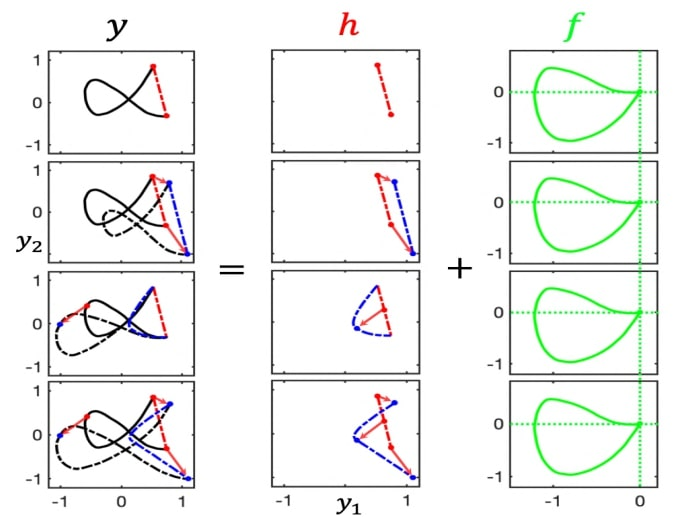
\includegraphics[width=0.7\textwidth]{figures/images/vmp/vmp.jpg}
    \caption{Graphical representation of the idea behind VMP \cite{zhou2019learning}. The final trajectory \( y \) is represented as the sum of two components: the elementary trajectory \( h \), and the shape modulation \( f \). The elementary trajectory can directly connect two points (e.g., start and goal points) with a linear segment.}
    \label{fig:vmp}
\end{figure}


In this framework, the learning procedure consists of two main components:
\begin{enumerate}
    \item \textbf{Learning the shape modulation}, which involves learning the prior probability distribution of the parameter vectors \( w \), characterized by the mean \( \mu_{w} \) and variance \( \Sigma_{w} \).
    \item \textbf{Modifying the elementary trajectory}, which entails determining whether the requested via-point can be accommodated by adjusting the shape modulation or by introducing a new linear segment into the elementary trajectory.
\end{enumerate}

To achieve this, VMP calculates the conditional probability of the shape modulation parameters given the desired via-point. If this probability exceeds a certain threshold \( \eta \), the shape modulation is adjusted to ensure the trajectory passes through the via-point. However, if the probability is below \( \eta \), indicating that the desired via-point is unlikely based on the learned prior probability of \( w \), VMP will modify the elementary trajectory instead.

Overall, the VMP framework enhances the adaptability of movement primitives by enabling the robot to learn and adjust its trajectories based on a limited number of demonstrations and specified via-points, making it a practical solution for various robotic applications.

In addition to these methodological advancements, several works have leveraged DMPs to solve specific robot manipulation problems \cite{meier2011movement_primitive,caccavale2019kinesthetic,agostini2020manipulation}. In all of these cited works, DMPs have been employed to address the problem of task decomposition, specifically the identification of different skills (e.g., pick, pour, place, reach, etc.) involved in a task. 

For instance, in the preliminary work \cite{meier2011movement_primitive}, the authors used a set of predefined motion primitives modeled as DMPs. The objective was to recognize these primitives within the demonstrated trajectory using an Expectation-Maximization algorithm. Similarly, in \cite{caccavale2019kinesthetic}, DMPs were utilized to learn and reproduce motion primitives from demonstrations during the kinesthetic teaching of structured tasks. In this work, action segmentation was performed based on either object proximity or explicit human commands. When the robot manager identifies a new action, the corresponding DMP is learned, and the sequence of tasks is organized into a hierarchical structure.

Despite all the successfully applications saw previsously, DMPs and all the variants have a very relevant limitation, that is related to the difficulty of handling high-dimensional input such as images. For this reason, the scientific community has focused the attention on methods that leverage deep architecture, that will be explained in detail in the following paragraphs.

\paragraph*{Single-Task Imitation Learning}\mbox{}\\
This paragraph will review the research conducted in the context of Single-Task Imitation Learning. Specifically, within the scope of robotic manipulation problems, the term ``Single-Task" indicates that the learned policy $\pi^{L}$ can perform only the specific task it has been trained on. For example, if the task involves a pick-and-place operation with a fixed place position, the model cannot handle variations in the place location. Additionally, the focus will be primarily on methods that use high-level state representations, such as images, processed by deep architectures to solve the problem.

In this scenario, the scientific literature extends far back in time. One of the seminal works in this field was proposed in 1988 by Pomerleau, who introduced \textit{ALVINN} \cite{pomerleau1988alvinn}. ALVINN is an autonomous vehicle driving system based on a Neural Network that predicts the steering angle from a synthetic camera image input. The network was trained on pairs of (image, steering angle), with the training procedure framed as a supervised classification problem. This was achieved by discretizing the steering angle into 45 units. Pomerleau's work immediately highlighted the issue of \textbf{compounding error}, which arises from the \textbf{covariate shift phenomenon}. This issue occurs because an action $a_{t}$ influences the subsequent state $s_{t+1}$, which becomes the next sample, thereby violating the i.i.d. assumption of Supervised Learning. This results in a test-data distribution that may differ from the training one. This phenomenon has significant consequences on the expected performance of the system and is addressed by methods discussed in the section on \textit{Interactive Imitation Learning}.

Despite the covariate-shift problem, \cite{zhang2018deep_vr_teleoperation} showed that very interesting performance can be obtained in the context of Robot Manipulation, by means of Behavioral Cloning and high quality demonstrations given by teleportation system. In this work, a Convolutional Neural Network was trained to predict the desired linear-velocity, angular-velocity of the end-effector, and the binary gripper state (open/close), given in input the current RGB-D observation of the scene, and the position of three points of the end-effector, during the last 5 time-steps (Figure \ref{fig:deep_bc}). The system was tested on 10 tasks, and the performance are reported in Table \ref{table:deep_vr_teleoperation_results}. The proposed system achieved a high success rate while evaluating all the tasks. The tests were carried out from different initial conditions but still quite similar to those present in the training set (e.g., the initial object positions have been uniformly distributed within the training regime, with random local variations around these positions). The analysis of failure cases showed that the leading cause of errors was the inability to detect critical points in the task execution, such as closing/opening the gripper to pick/place the object or detect the position of the object of interest in order to avoid collision with it.
% What Matters in Learning from Offline Human Demonstrations for Robot Manipulation
% Behavior Transformers
% Learning Latent Plans from Play
% Waypoint-Based Imitation Learning for Robotic Manipulation
% Imitating Task and Motion Planning with Visuomotor Transformers
% Implicit Behavioral Cloning
% Deep imitation learning for bimanual robotic manipulation
\textcolor{red}{ToContinue} 
\begin{figure}[bt]
    \centering
    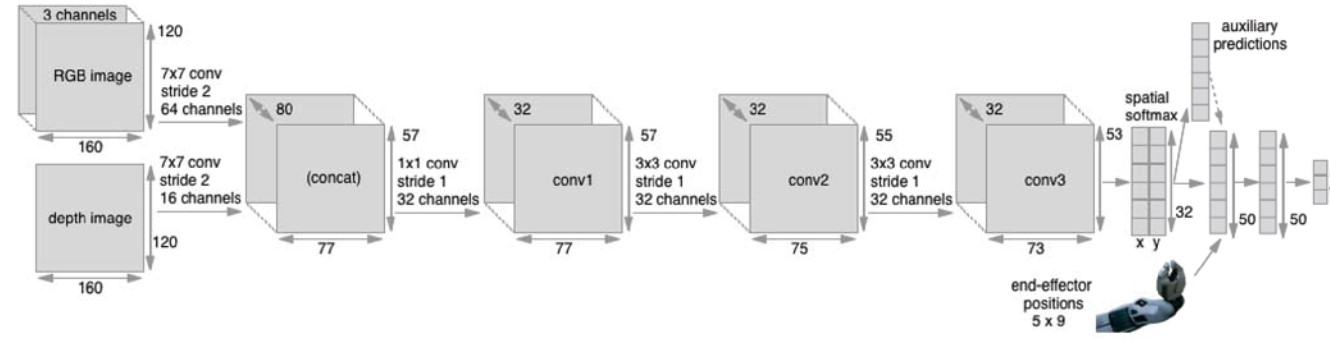
\includegraphics[width=0.9\textwidth]{figures/images/deep_imitation_bc/deep_imitation_bc.jpg}
    \caption{Architecture proposed in~\cite{zhang2018deep_vr_teleoperation}}
    \label{fig:deep_bc}
\end{figure}

% \usepackage{graphicx}
% \usepackage{hhline}


\begin{table}
    \centering
    \caption{Statistics of Training set, and Test Success rate~\cite{zhang2018deep_vr_teleoperation}}
    \label{table:deep_vr_teleoperation_results}
    \resizebox{\linewidth}{!}{%
    \begin{tabular}{|c|c|c|c|c|c|c|c|c|c|c|} 
    \hline
    \textbf{Task} & \textbf{Reaching} & \textbf{Grasping} & \textbf{Pushing} & \textbf{Plane} & \textbf{Cube} & \textbf{Nail} & \begin{tabular}[c]{@{}c@{}}\textbf{Grasp-}\\\textbf{and-}\\\textbf{Place}\end{tabular} & \begin{tabular}[c]{@{}c@{}}\textbf{Grasp-}\\\textbf{Drop-}\\\textbf{Push}\end{tabular} & \begin{tabular}[c]{@{}c@{}}\textbf{Grasp-}\\\textbf{Place-x2}\end{tabular} & \textbf{Cloth} \\ 
    \hhline{|===========|}
    \#demo & 200 & 180 & 175 & 319 & 206 & 215 & 109 & 100 & 60 & 100 \\ 
    \hline
    \begin{tabular}[c]{@{}c@{}}demo duration \\(min)\end{tabular} & 13.7 & 11.1 & 16.9 & 25.0 & 12.7 & 13.6 & 12.3 & 14.5 & 11.6 & 10.1 \\ 
    \hline
    \begin{tabular}[c]{@{}c@{}}Test success rate\\(\%)\end{tabular} & 91.6 & 97.2 & 98.9 & 87.5 & 85.7 & 87.5 & 96.0 & 83.3 & 80.0 & 97.4 \\
    \hline
    \end{tabular}
    }
    \end{table}
\paragraph*{Interactive Imitation Learning}\mbox{}\\
The Interactive Imitation Learning approach encompasses all methods specifically designed to address or mitigate the compounding error phenomenon, which was first described in~\cite{pomerleau1988alvinn}.

As previously mentioned, this issue arises because, although Behavioral Cloning primarily follows a supervised learning procedure, it does not satisfy the i.i.d. assumption. The agent's actions influence subsequent observations, creating dependencies between samples in the training set. Consequently, when the agent interacts with the environment, even small errors can lead to new observations outside the training distribution, potentially resulting in an unrecoverable situation that the robot cannot resolve autonomously.

The significance of this problem was first formalized in \cite{ross2010efficient_reductions}. The authors observed that if a system makes an error with probability $\epsilon$ in a task with a time horizon of $T$, then, due to the compounding of errors, a supervised learner incurs a quadratic total cost of $O(\epsilon \ T^{2})$, instead of the expected linear cost of $O(\epsilon \ T)$. The quadratic term arises because, at any given time step $t$, the agent's state is influenced by errors made in the previous $t-1$ steps. This cumulative effect breaks the independence assumption typically held in the i.i.d. setting.

To attenuate this problem, \textbf{interactive supervised learning algorithms} have been proposed, such as the well-known \textit{DAgger} \cite{ross2011dagger}. Algorithm \ref{alg:dagger} describes the DAgger procedure. It is an aggregation strategy, based on the idea to train the policy $\pi^{L}$ under the state-distribution induced by the policy itself, but with the correct action performed by the expert. The main problem with DAgger is that it requires the expert to interact with the system during the training, introducing both \textbf{safety} and \textbf{data-efficiency} problems, especially when the system does not provide the human expert with sufficient control authority during the sampling process \cite{laskey2017comparing_hc_rc}. 
\begin{algorithm}
\caption{DAgger Algorithm \cite{ross2011dagger}}\label{alg:dagger}
\begin{algorithmic}
\Require Initial Dataset $\mathcal{D} \leftarrow \emptyset$, Initial policy $\pi^{L}_{1}$
\Ensure The best policy $\pi^{L}_{i}$
\For {$i=1, \dots N$}
    \State Sample $T-step$ trajectories using $\pi^{L}_{i}$
    \State Let $\mathcal{D}_{i} = {(s_{t}, \pi^{E}(s_{t}))}$, state $s_{t}$ visited by policy $\pi^{L}_{i}$, and actions given by the expert
    \State Aggregate Dataset, $\mathcal{D} \leftarrow \mathcal{D} \bigcup \mathcal{D}_{i}$
    \State Train policy $\pi^{L}_{i}$ on $\mathcal{D}$
    \State Let $\pi^{L}_{i+1} = \beta_{i}\pi^{E} + (1- \beta_{i})\pi^{L}_{i}$
\EndFor
\end{algorithmic}
\end{algorithm}

Human-Guided DAgger (HG-DAgger) \cite{kelly2019hg_dagger} is an enhancement of the traditional DAgger strategy, where a human expert oversees the rollout of the current policy. If the agent moves into an unsafe region of the state space, the expert steps in to guide the system back to safety. Specifically, HG-DAgger was proposed in the context of autonomous vehicle driving, however, in \cite{jang2022bc_z}, it was shown that HG-DAgger is particularly effective in robotic manipulation tasks. The study found that, given the same total number of episodes, a policy trained exclusively on expert demonstrations has a significantly lower success rate than one trained on a dataset that includes both expert demonstrations and expert corrections.

In the context of Interactive Learning for Robot Manipulation, other works of interest include \cite{mandlekar2020human_in_the_loop,chisari2022correct}. 

In \cite{chisari2022correct}, a human expert provides both \textbf{corrective} and \textbf{evaluative} feedback. The former consists in the human that takes control of the robot to adjust the trajectory, the latter consists in a scalar weight $q$, set to 1 if the trajectory is satisfactory, 0 if the trajectory is not satisfactory, $\alpha$ if the trajectory is adjusted by the expert, where $\alpha$ is the ratio between non-corrected and corrected samples. Then a Neural Network was trained by minimizing a weighted version of the maximum-likelihood, $\mathcal{L}(a_{t},s_{t}) = - q \ log(\pi^{L}_{\theta}(a_{t}|s_{t}))$. Real-world experiments show that with a training time of \textbf{41 minutes}, including environmental reset, it was possible to have an agent capable of performing tasks such as picking up a cube or pulling a plug.
\paragraph*{Multi-Task Imitation Learning}\mbox{}\\
The methods discussed in the previous paragraphs describe architectures and approaches specifically designed to solve a single task, with limited generalization to the object's category (e.g., picking blocks rather than balls) and initial state (e.g., the object's starting position). For instance, a system trained for pick-and-place operations cannot be repurposed for tasks like assembly operations. The methods described in this paragraph address these limitations, solving the problem of \textit{Multi-Task Imitation Learning} (MTIL)

Before starting to present and describe the different methods and approaches, it is necessary to describe the problem. Starting from a reformulation of the dataset used to train the system and the learned policy.
Indeed, in Section~\ref{sec:problem_formulation}, the expert dataset $\mathcal{D}^{E}$ has been introduced. Based on the problem to solve this dataset can composed in different way. Specifically, in the context of MTIL, the dataset $\mathcal{D}^{E}$ can be seen as a composition of $n$ datasets, $\mathcal{D}^{E}=\left \{\mathcal{D}_{1}, \dots, \mathcal{D}_{n}\right \}$, where $\mathcal{D}_{i} = \left \{ (\tau_{m_{i}}^{j}, \ c_{m_{i}}), j=1,\dots,N, \ m_{i} \in \mathcal{M}_{i}\right \}$ is the \textit{single-task dataset}, composed of:
\begin{itemize}
    \item $N$ expert demonstration for each $m^{th}$ variation of the $i^{th}$ task, where $M_{i}$ is the number of variation for the $i^{th}$ task.
    \item Agent trajectories $\tau_{m_{i}}^{j} = (s_{0}, a_{0}, s_{1}, a_{1}, \dots, a_{T-1}, s_{T})$. where $s_{t}$ is the state at time $t$ and $a_{t}$ is the corresponding action (Section \ref{sec:problem_formulation}).
    \item Task-conditioning signal $c_{m_{i}}$ for the $m^{th}$ variation of $i^{th}$ task, which describes the desired task in terms of video demonstrations \cite{james2018task_embedded,bhutani2022attentive_one_shot,dasari2021transformers_one_shot,mandi2022towards_more_generalizable_one_shot}, natural language description \cite{stepputtis2020language,jang2022bc_z,mees2022calvin,doasIcan2022,mees2022hulc,brohan2022rt,shridhar2023perceiver} or multi-modal prompt, that exploits both visual information (e.g., an image of the target object) and text information that contains the information related to the action to be performed \cite{jiang2023vima}.
\end{itemize}
The goal of Multi-Task Imitation Learning is to learn a \textit{conditioned policy} $\pi^{L}_{\theta}(a_{t}|s_{t}, c_{m_{i}})$, that is able to map the current state and command into the corresponding action.
Depending on how the policy is defined, various loss functions come into play. In the case of deterministic policies, the learning process focuses on minimizing the Mean-Squared Error (refer to Formula \ref{eq:mse}). However, for probabilistic policies, the learning process centers around minimizing the Negative Log-likelihood (refer to Formula \ref{eq:nll}). This approach aims to enhance the probability of correctly executing the action.
% \begin{equation}
%     \label{eq:mse}
%     \mathcal{L}(D^{E}, \pi^{L}_{\theta}) = \frac{1}{n} \sum_{\mathcal{D}^{i} \sim \mathcal{D}^{E}} \frac{1}{N} \sum_{(\tau_{m_{i}}^{j}, c_{m_{i}}) \sim \mathcal{D}^{i}} \frac{1}{T}\sum_{t=0}^{T} (a_{t} - \pi^{L}_{\theta}(s_{t}, c_{m_{i}}))
% \end{equation}
% \begin{equation}
%     \label{eq:nll}
%     \mathcal{L}(D^{E}, \pi^{L}_{\theta}) = \frac{1}{n} \sum_{\mathcal{D}^{i} \sim \mathcal{D}^{E}} \frac{1}{N} \sum_{(\tau_{m_{i}}^{j}, c_{m_{i}}) \sim \mathcal{D}^{i}} \frac{1}{T}\sum_{t=0}^{T} (a_{t} - \pi^{L}_{\theta}(s_{t}, c_{m_{i}}))
% \end{equation}

\begin{equation}
    \label{eq:mse}
    \mathcal{L}(\tau_{m_{i}}^{j}, c_{m_{i}},\pi^{L}_{\theta}) = \frac{1}{T}\sum_{t=0}^{T} (a_{t} - \pi^{L}_{\theta}(s_{t}, c_{m_{i}}))^{2}
\end{equation}
\begin{equation}
    \label{eq:nll}
    \mathcal{L}(\tau_{m_{i}}^{j}, c_{m_{i}},\pi^{L}_{\theta}) = - \frac{1}{T}\sum_{t=0}^{T} log(\pi^{L}_{\theta}(a_{t}|s_{t}, c_{m_{i}}))
\end{equation}
The following sections will describe the various approaches proposed to address the problem. Figure \ref{fig:mtil_taxonomy} illustrates the taxonomy used for the Multi-Task Imitation Learning methods. Specifically, the methods are categorized based on the type of generalization required by the algorithm (Few-Shot vs. Zero-Shot). For Few-Shot generalization, the Meta-Learning paradigm will be discussed, as it is most relevant to the problem at hand. For Zero-Shot generalization, the methods are further divided based on the type of conditioning signal used, whether it is provided through natural language descriptions or visual information.
\begin{figure}[t]
    \centering
    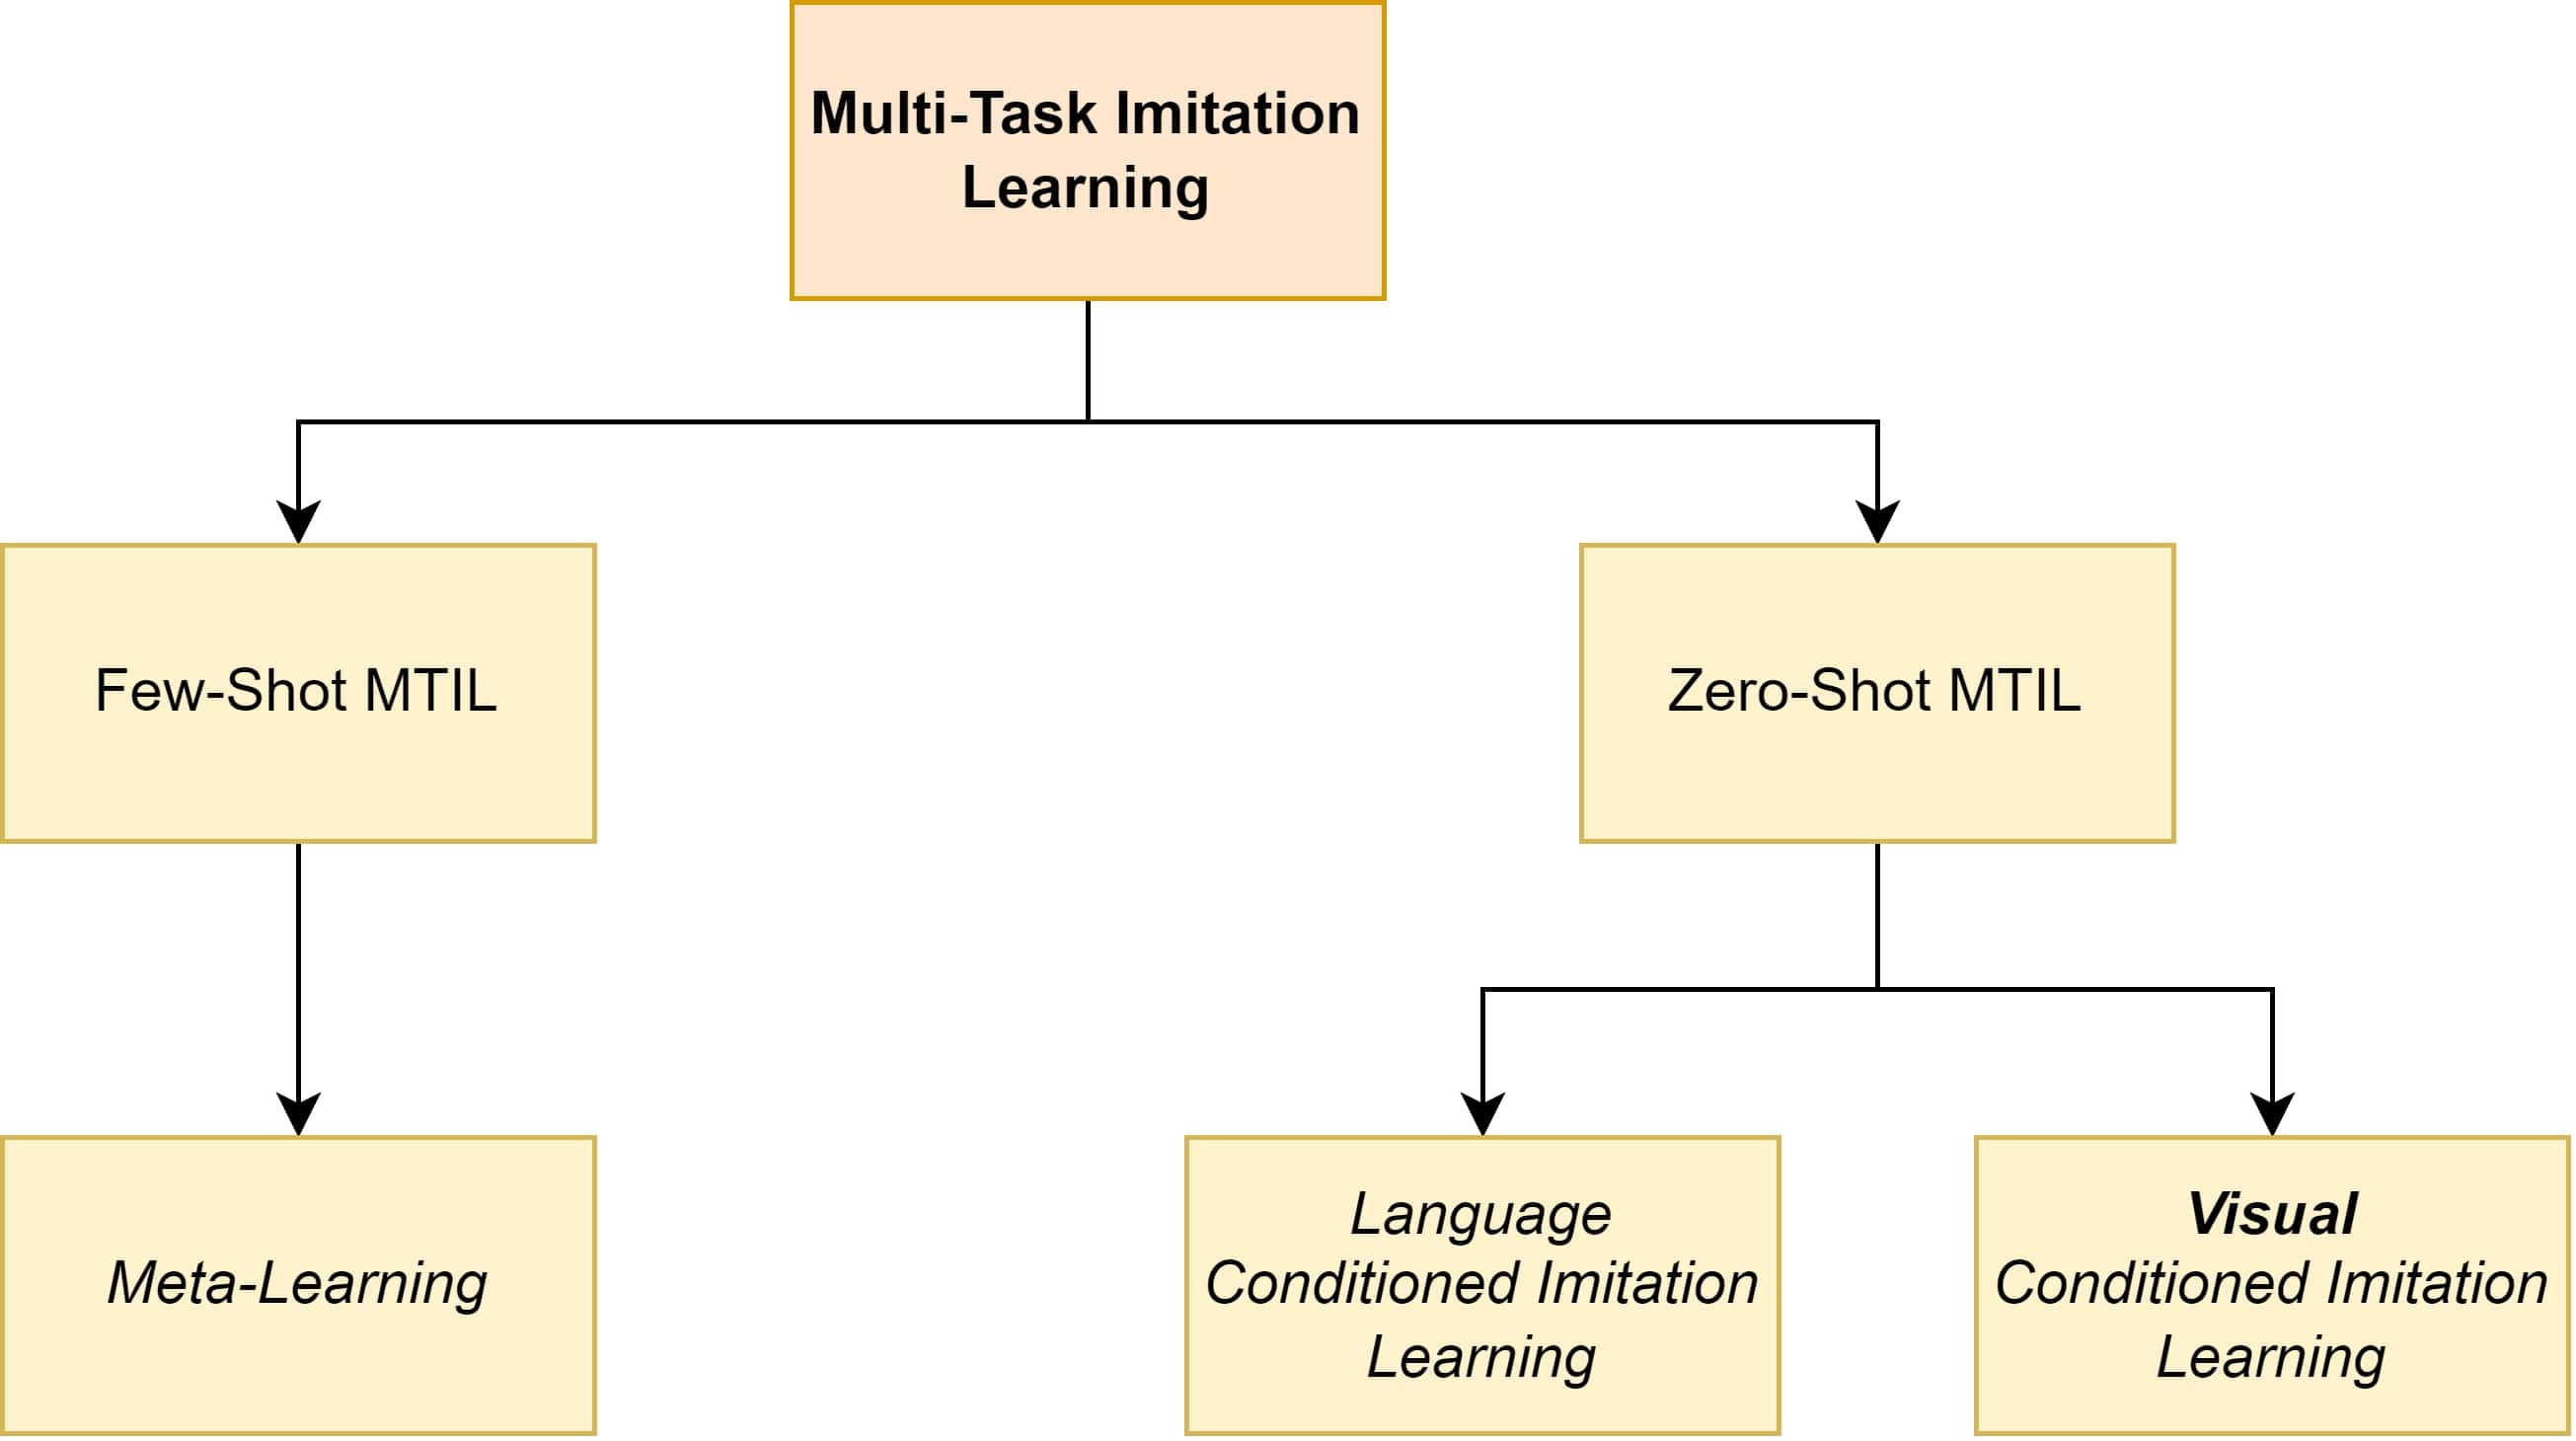
\includegraphics[width=0.8\textwidth]{figures/images/MTIL_taxonomy.jpg}
    \caption{Multi-Task Imitation Learning Taxonomy.}
    \label{fig:mtil_taxonomy}
    
\end{figure}


\textbf{Few-Shot MTIL} refers to approaches designed to train a model on a variety of tasks so that it can effectively solve a new task using only a small number of samples and consequently requires only a few back-propagation steps \cite{finn2017maml}. In this context, one of the most significant learning paradigms, especially relevant to robotic manipulation, is \textit{Meta-Learning}. The goal of Meta-Learning is to train a model that can ``learn to learn," meaning it develops a set of general weights $\theta$ that, while not directly usable for solving any specific task within a distribution of tasks $\mathcal{T}$, can be quickly adapted through a few backpropagation steps to solve a given task within that distribution, $\mathcal{T}_{i} \in \mathcal{T}$. One of the most popular Meta-Learning algorithms is the \textit{Model-Agnostic Meta-Learning} (MAML) algorithm \cite{finn2017maml}, described in Algorithm \ref{alg:maml}. The MAML algorithm follows an iterative learning procedure consisting of two steps:
\begin{itemize}
    \item \textbf{Meta-Learning}: During this phase, task-specific weights $\theta_{i}$ are computed for each sampled task $\mathcal{T}_{i}$. Specifically, the \textit{meta-parameters} $\theta$ are updated according to the gradient obtained from evaluating the loss function on the $i^{th}$ task $\mathcal{T}_{i}$, where the function $f$ is parameterized by the meta-parameters $\theta$.

    \item \textbf{Meta-Adaptation}: In this phase, the meta-parameters are further refined. The loss function $f$, now parameterized by the task-specific parameters for the $i^{th}$ task, is used to adjust the meta-parameters based on the gradients derived from the sum of the loss functions evaluated on the task-specific weights. This process provides feedback to the meta-parameters $\theta$ from each task, leading to a generalized point that can be easily adapted to new tasks (Figure \ref{fig:maml_weights}).
\end{itemize}
\begin{algorithm}[t]
\caption{Model-Agnostic Meta-Learning (MAML) \cite{finn2017maml}}
\label{alg:maml}
\begin{algorithmic}
\REQUIRE Distribution over tasks $p(\mathcal{T})$
\STATE Randomly initialize $\theta$
\WHILE {$i=1, \dots N$}
    \STATE Sample batch of tasks $ \mathcal{T}_{i} \sim p(\mathcal{T})$
    \FOR {\textbf{all} $\mathcal{T}_{i}$}
        \STATE Evaluate $\nabla_\theta \mathcal{L}_{\mathcal{T}_{i}}(f_{\theta})$ w.r.t. $K$ examples
        \STATE Compute adapted parameters with gradient descent: $\theta'_{i} = \theta - \alpha \nabla_\theta\mathcal{L}_{\mathcal{T}_{i}}(f_{\theta})$
    \ENDFOR
    \STATE Update $\theta \leftarrow \theta - \beta \nabla_\theta \sum_{\mathcal{T}_{i} \sim p(\mathcal{T})} \mathcal{L}_{\mathcal{T}_{i}}(f_{\theta'_{i}})$
\ENDWHILE
\end{algorithmic}
\end{algorithm}
\begin{figure}[tb]
    \centering
    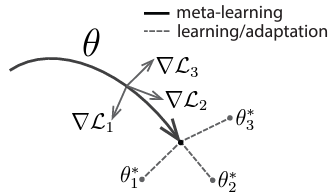
\includegraphics[width=0.6\textwidth]{figures/images/maml_weights.png}
    \caption{Diagram of MAML algorithm, which optimizes for a representation $\theta$ that can quickly adapt to new tasks}
    \label{fig:maml_weights}
\end{figure}

The MAML algorithm is the base for different methods which apply Few-Shot Imitation Learning in the context of Behavioral Cloning \cite{finn2017one_shot_visual_il,yu2018daml,yu2018one_shot_hil}.

In \cite{finn2017one_shot_visual_il}, MAML algorithm was used to prove the effectiveness of Meta-Learning in the context of real robot manipulation, with visual observations, as opposite to \cite{duan2017one_shot_il}. A Convolutional Neural Network was trained by following the Algorithm \ref{alg:maml}, using as loss-function the Mean Squared Error, computed between the predicted action and the ground truth one. For real-robot experiments a dataset of \textbf{1300} placing demonstrations (i.e., place an holded object in a target container), containing near to \textbf{100} different objects, was collected through teleportation. The trained system was tested by performing the adaptation step on one video demonstration, over 29 new objects, moreover, between the video demonstration and the actual execution, the objects configuration was changed. In this setting the system reached the $\mathbf{90\%}$ of success rate, outperforming baseline methods based on LSTM \cite{duan2017one_shot_il}, and contextual network (i.e., a Convolutional Neural Network that takes in input the current observation and the image representing the target state).

In \cite{yu2018daml}, the \textit{Domain Adaptive Meta-Learning} algorithm (DAML) was proposed with the goal of learning to infer a policy from a single human demonstration. To achieve it, a two-step algorithm was proposed. In the first-step, called \textbf{Meta-Learning step}, given in input, for each task $\mathcal{T}$, a set of human demo $\mathcal{D}^{h}_{\mathcal{T}}$ and a set or robot demo $\mathcal{D}^{r}_{\mathcal{T}}$ (Figure \ref{fig:daml_tasks}), the \textit{initial policy parameters} $\theta$ and the \textit{adaptive loss} parameters $\psi$ are learned, solving the problem in Formula \ref{eq:daml}.
\begin{equation}
 \label{eq:daml}
 \underset{\theta,\psi}{\min} \sum_{\mathcal{T} \sim p(\mathcal{T})} \sum_{\mathbf{d}^{h} \sim D^{h}_{\mathcal{T}}} \sum_{\mathbf{d}{^r} \sim D^{r}_{\mathcal{T}}} \mathcal{L}_{BC}(\theta - \alpha \nabla_\theta\mathcal{L}_{\psi}(\theta,\mathbf{d}^{h}), \mathbf{d}^{r})
\end{equation}

\newline The outer loss is the classic supervised Behavioral Cloning loss, defined as $\mathcal{L}_{BC}(\phi, \mathbf{d^{r}}) = \sum_{t} \log(\pi_{\phi}(a_{t} \mid s_{t}, o_{t}))$. The inner loss, $\mathcal{L}_{\psi}$, is a learned \textbf{adaptive loss}. Specifically, $\mathcal{L}_{\psi}$ is used during Meta-Adaptation, where the policy parameters are updated by evaluating the gradients derived from $\mathcal{L}_{\psi}$. This process involves using a video of a human demonstrating a new task $\mathcal{T}$ as input, leading to the policy update defined by $\phi_{\mathcal{T}} = \theta - \alpha \nabla_{\theta} \mathcal{L}_{\psi}(\theta, \mathbf{d}^{h})$. 
\newline This adaptive loss is the key component proposed in DAML. To use it effectively, it is necessary to learn the parameters $\psi$, observing how there is no direct correspondence between the human video demonstration and the robot's ground truth actions. To address this challenge, the authors of DAML observed that while the policy learns to produce appropriate actions through the $\mathcal{L}_{BC}$ loss, the adaptive loss should instead adjust the perceptual aspect of the policy, focusing on human motion and the manipulated object. Based on this insight, the authors implemented the function $\mathcal{L}_{\psi}$ using a 1D Temporal Convolutional Network (Figure \ref{fig:daml_temporal_adaptation_loss}). The convolutional layers are applied to a stack of embeddings generated by the policy $\pi$ across different frames of the video demonstrations. The parameters of this module are learned during the meta-training phase, following the weight update process described in Formula \ref{eq:daml_temporal_adaptation_loss}. The objective of $\mathcal{L}_{\psi}$ is to generate task-specific policy parameters $\phi_{\mathcal{T}}$ that guide the policy to produce effective actions.

\begin{equation}
 \label{eq:daml_temporal_adaptation_loss}
 \begin{matrix}
    (\theta, \psi) \leftarrow(\theta, \psi)-\beta \nabla_{\theta, \psi} \mathcal{L}_{\mathrm{BC}}\left(\phi_{\mathcal{T}}, \mathbf{d}^r\right) \\ \\
   \phi_{\mathcal{T}}=\theta-\alpha \nabla_\theta \mathcal{L}_\psi\left(\theta, \mathbf{d}^h\right)
   \end{matrix}
\end{equation}

\newline Experimental evaluation on tasks such as placing, pushing, and pick-and-place, has shown that: \begin{itemize}
    \item The system was able to generalize across both new objects and objects configuration starting from only a single human demonstration;
    \item A performance degradation was observed in large domain-shift experiments, such as novel backgrounds and different camera view-points.
\end{itemize}
\begin{figure}[t]
    \centering
    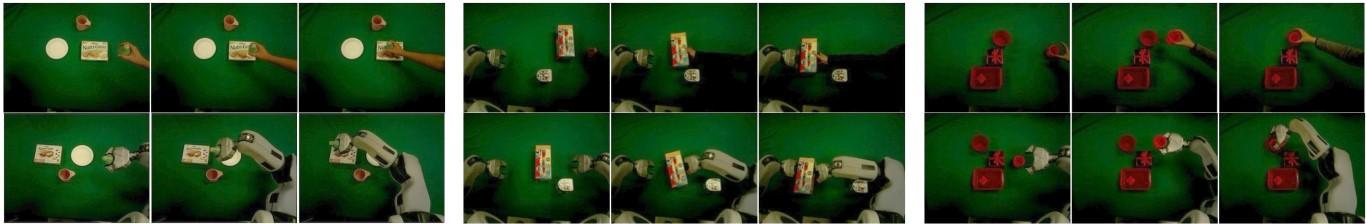
\includegraphics[width=\textwidth]{figures/images/daml/tasks.jpg}
    \caption{Tasks performed in \cite{yu2018daml}. (Top row) Human demonstration, (Bottom row) robot demonstration. (Left) Placing task, (Middle) pushing task, (Right) pick-and-place task.}
    \label{fig:daml_tasks}
\end{figure}

\begin{figure}[t]
    \centering
    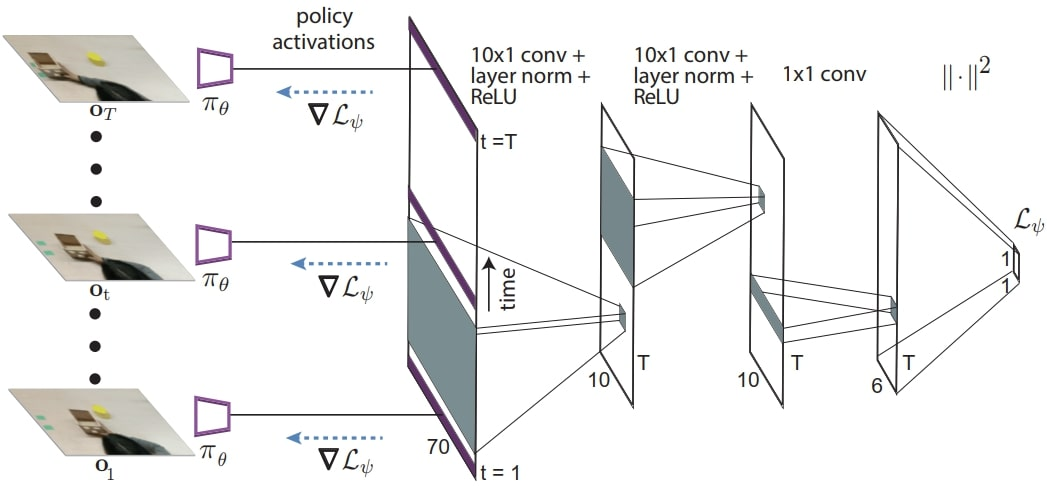
\includegraphics[width=0.8\textwidth]{figures/images/daml/daml_temporal_adaptation_loss.jpg}
    \caption{The Temporal Adaptation Loss architecture applies 1D temporal convolutional layers to the stacked embeddings generated by the policy $\pi$ from the frames of the human video demonstration.}
    \label{fig:daml_temporal_adaptation_loss}
\end{figure}

Meta-Learning algorithms have demonstrated intriguing properties, notably their capacity for few-shot generalization to novel objects and object configurations. However, it has been observed that during the adaptation step, these methods tend to lose their effectiveness in performing other tasks. This limitation has underscored the need for the development of Multi-Task Imitation Learning methods, which aim to address these shortcomings and enable more versatile task execution in complex scenarios. These kind of methods will be discussed in the following paragraphs.

\textbf{Zero-Shot MTIL} refers to approaches that aim to train a model capable of solving different tasks without any further adaptation or backpropagation steps. This approach addresses a key issue in Meta-Learning methods, which is the problem of forgetting how to solve previous tasks after adapting to a new one. The goal is to develop a single policy that can handle multiple tasks in a zero-shot manner.

In this context, a crucial design choice is how to convey the desired task to the policy. The literature identifies two main methods to address this problem:

\begin{enumerate}
    \item \textit{Language Conditioned}: These methods leverage natural language descriptions of tasks to inform the model about the task to be executed.
    \item \textit{Visual Conditioned}: These methods use visual information (e.g., goal-state images, video demonstrations) to provide the model with the task instructions.
\end{enumerate}
\textcolor{red}{ToDo}

\textit{Language Conditioned}

\textit{Visual Conditioned}
\paragraph*{Object-Oriented Imitation Learning}\mbox{}\\
All the methods discussed so far share a common characteristic: they are end-to-end systems that take high-level inputs, such as images, and directly generate the corresponding actions as output. While this approach can be sufficient in scenarios where the scene is simple, meaning there are no distracting objects, or if there are distracting objects, they can be easily identified by the system because they are consistently not involved in the manipulation, this end-to-end approach may struggle in more complex environments. Specifically, it can encounter difficulties when the robot workspace contains objects that are similar to each other, especially if these objects are involved in manipulation for some task variations.

Based on this consideration, this paragraph will describe methods that leverage \textbf{object priors}. Specifically, leveraging object priors means that the control policy is informed not only by the embedding of the agent scene, which is obtained from a deep architecture, but also by object-level information, such as the bounding boxes of objects in the scene, obtained from an object detector.

The concept of leveraging object priors has been explored in both earlier works \cite{devin2018deep,park2021object} and more recent approaches \cite{belkhale2023plato,zhu2023viola,zhu2023learning,jiang2023vima}.

One of the preliminary works on leveraging object priors was presented by the authors of \cite{devin2018deep}. This work primarily focuses on the challenge of generalization in Learning from Demonstration (LfD) systems that use an end-to-end approach. In such systems, a task-specific model is trained to predict actions based on raw visual observations. The authors found that while it is possible to achieve good \textit{instance-level generalization}, meaning the model can solve tasks with varying initial configurations using a limited number of samples, achieving \textit{category-level generalization} is more challenging. Category-level generalization refers to the model ability to solve tasks involving different objects. To achieve this, the dataset must include a large number of trajectories involving a wide variety of objects. For instance, if the task is to pour the contents of a bottle into a cup, the dataset should contain trajectories with different types of cups and bottles. However, constructing such a dataset is time-consuming and costly. Moreover, the potential of well-known large datasets in classical computer vision tasks, such as object detection, is not fully utilized.

To address this issue, the authors proposed a paradigm shift by introducing a robotic vision framework that operates on sets of objects rather than raw pixel data. This framework leverages prior datasets to learn a generic object concept model, thereby enhancing category-level generalization without requiring an extensive and diverse dataset. The framework is illustrated in Figure \ref{fig:object_prior_framework} and is composed of several stages:
\begin{itemize}
    \item \textbf{Meta-Attention}, which is basically a Region Proposal Network (RPN) \cite{fastrcnn}, trained on the well known MSCOCO \cite{lin2014microsoft} dataset. The RPN generates objects proposals, i.e., region of the image that possibly contain an object.
    \item \textbf{Task-Specific Attention}, which aims to learn what are the object of interest with respect to the task in hand. This module is parametreized as a vector $w$ such that the attention paid to $o^i$ is proportional to $e^{w^Tf(o^i)}$.
    \item \textbf{Soft Attention}, this module gives a probabilistic meaning to the atttention map obtained from the Task-Specific Attention. Specifically, a Boltzmann distribution is used to map the attention weights to a probability for each object proposal, i.e., $p\left(o^i \mid w_j\right)=\frac{e^{w_j^{\top} \frac{f\left(o^i\right)}{\left\|f\left(o^i\right)\right\|_2}}}{\sum_{i=0}^N e^{w_j^{\top} \frac{f\left(o^i\right)}{\left\|f\left(o^i\right)\right\|_2}}}$.
    \item \textbf{Movement Prediction Network}, this module predicts the next robot action, given the attended object information from the soft attention, and the robot state represented by the joint and end-effector state.
\end{itemize}
\begin{figure}[t]
    \centering
    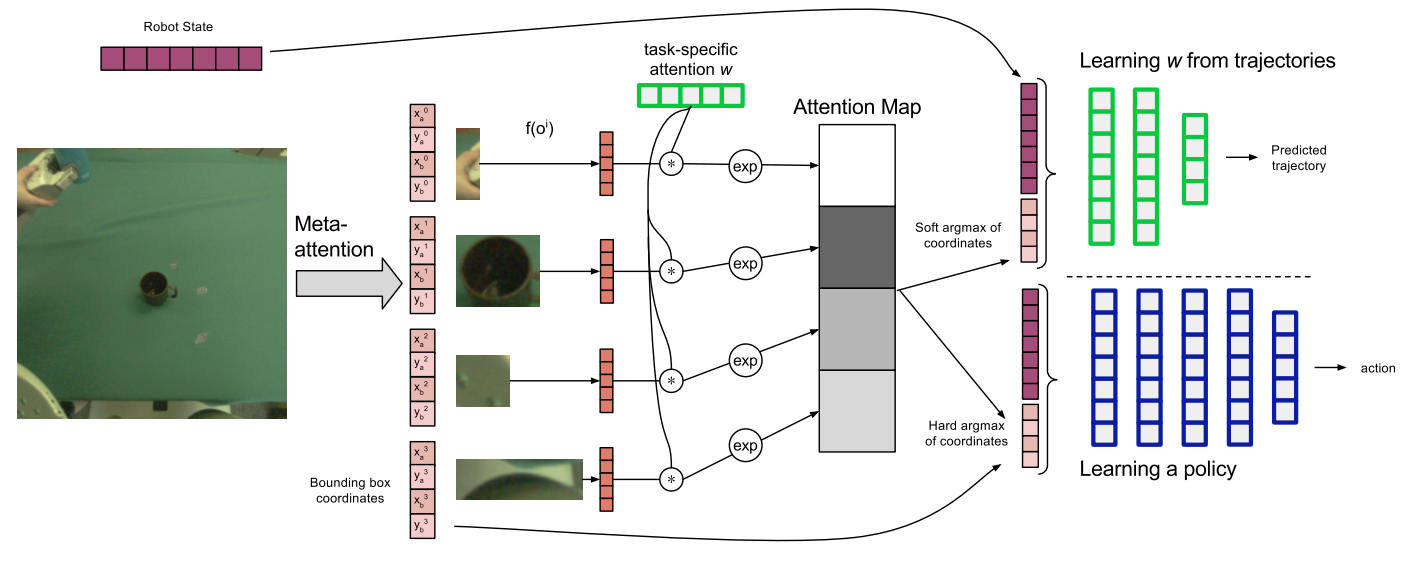
\includegraphics[width=0.8\textwidth]{figures/images/object_prior_framework.png}
    \caption{
            Robotic vision framework proposed in \cite{devin2018deep}. The framework is divided into different stages: \textbf{Meta-Attention}: Generates object proposals from an input image, trained on an object detection dataset, and shared across tasks; \textbf{Task-Specific Attention}: Focuses on relevant objects for a task using the meta-attention's semantic features; \textbf{Soft Attention}: Distributes attention as probabilities over object proposals using a Boltzmann distribution; \textbf{Movement Prediction Network}: Combines attended object information with the robot's state to predict the next action.
        }
    \label{fig:object_prior_framework}
\end{figure}
This preliminary work focused mainly on two tasks:
\begin{itemize*}
    \item  \textit{Pouring Task}: The robot is required to pour contents from a bottle into a mug. The challenge is to locate the mug from an image without being explicitly provided its location, especially when different mugs are used during training and testing.
    \item \textit{Sweeping Task}: The robot must sweep an object (e.g., a plastic orange) into a dustpan, with both objects starting in different positions. This task requires the robot to adapt its approach based on the relative positions of the objects.
\end{itemize*}
During testing, the authors focused on \textit{Category Generalization} and the ability to \textit{Ignore Distractor Objects}. For the former, the system was trained with only one type of mug and evaluated with other mugs (Figure \ref{fig:pouring_task_setting}). The results showed that the system successfully poured the contents into the correct mug, thanks to the learned task-specific attention weight that highlighted the mug features. For the latter, the authors designed a test where two mugs were present in the scene (Figure \ref{fig:task_specific_attention}). Since the model did not receive any conditioning signal indicating which mug to use, the authors fine-tuned the attention weight on trajectories where only the brown mug was used, demonstrating that this mechanism could focus on more specific features, such as the mug color.
\begin{figure}[t]
    \centering
    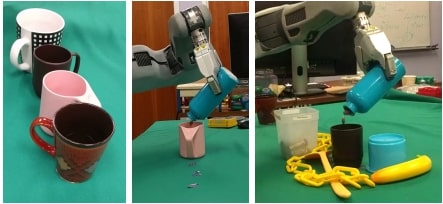
\includegraphics[width=0.6\textwidth]{figures/images/deep_object_centric_representation/pouring_task.jpg}
    \caption{Pouring task setting proposed in \cite{devin2018deep}. (Left) Mugs used for evaluation. Note that only the brown mug was seen during training. Center: Successful pouring into the pink mug. (Right) Pouring into the brown mug in a cluttered environment that was not seen during training.}
    \label{fig:pouring_task_setting}
\end{figure}

\begin{figure}[t]
    \centering
    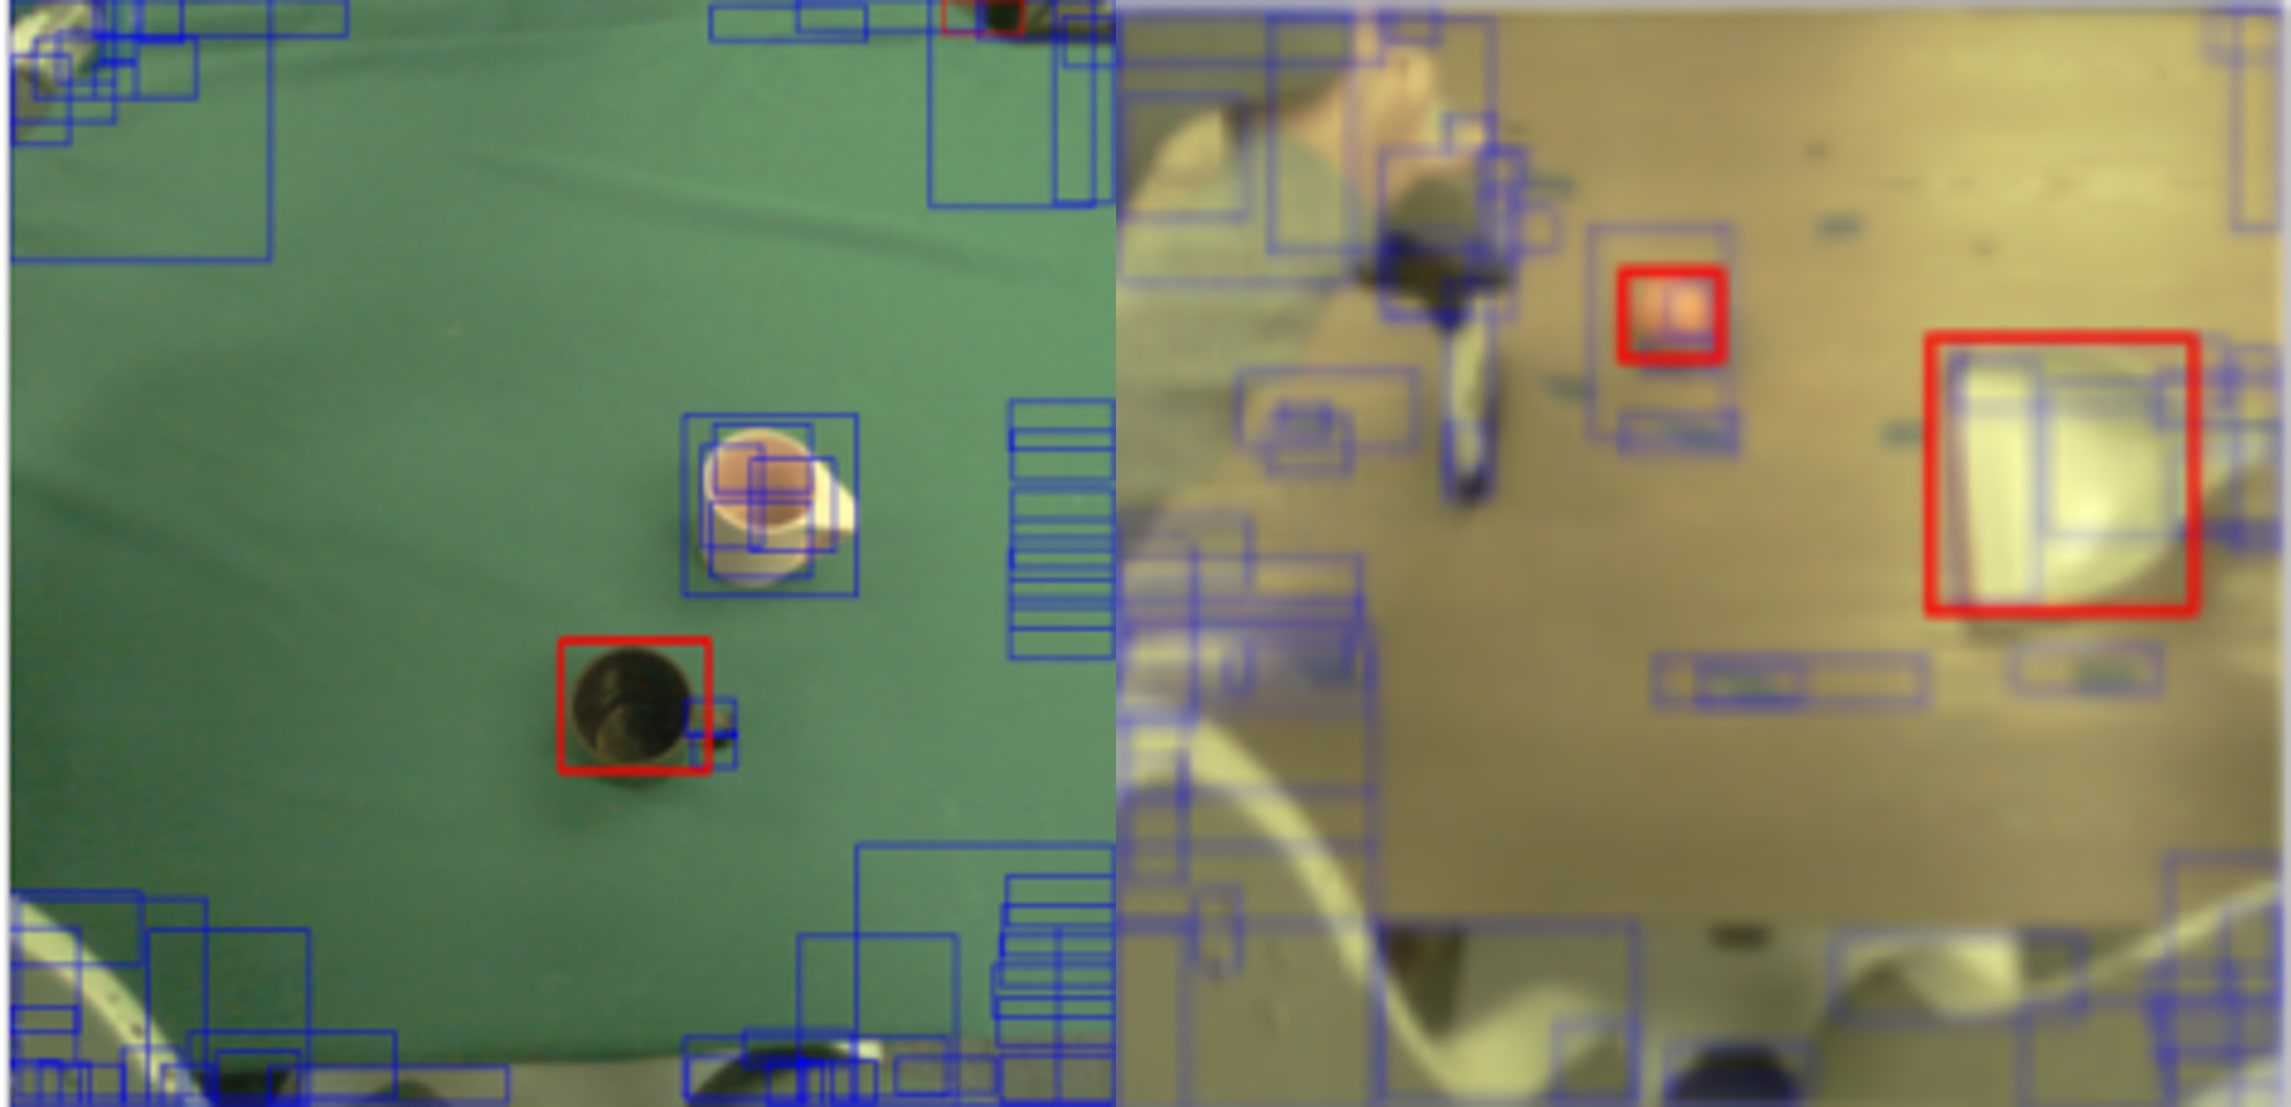
\includegraphics[width=0.6\textwidth]{figures/images/deep_object_centric_representation/mugs_distractors.jpg}
        \caption{The region proposals (meta-attention) are drawn in blue and the task-specific attended regions are drawn in red. For the Pouring task with distractor mug (pink) and target mug (brown), the attention locks on to the brown mug as its position defines the trajectory. For the sweeping task, two attention vectors are used, one attends to the orange and one attends to the dustpan.}
    \label{fig:task_specific_attention}
\end{figure}

In summary, this preliminary work demonstrated that leveraging object priors can facilitate category-level generalization by utilizing large, well-known datasets for the object-detection problem. However, the experimental setup was relatively simple, even in scenarios with distractor objects. The proposed system could handle distractor objects only after specific fine-tuning and was not able to dynamically discriminate between objects of interest and distractors based on task variations.

A recent work that follows a similar approach is proposed in \cite{zhu2023viola}. In this work, the authors introduced VIOLA (Visuomotor Imitation via Object-centric Learning) (Figure \ref{fig:viola_architecture}), an architecture inspired by the ideas presented in \cite{devin2018deep}. VIOLA uses an RPN and a ResNet18 \cite{resnet} to generate object proposals and produce a spatial feature map, respectively. It then constructs a \textit{per-step feature} vector, composed of three key elements: a \textbf{global context feature} that encodes the current task stage, an \textbf{eye-in-hand visual feature} to mitigate occlusion, and a \textbf{proprioceptive feature} that captures the robot state. These per-step features are concatenated to form a \textbf{history of observations}, which is designed to capture temporal dependencies and dynamic changes in object states. This tensor is then fed into a Transformer \cite{vaswani2017attention}, which leverages its intrinsic attention mechanism to automatically focus on the object of interest.
\begin{figure}[t]
    \centering
    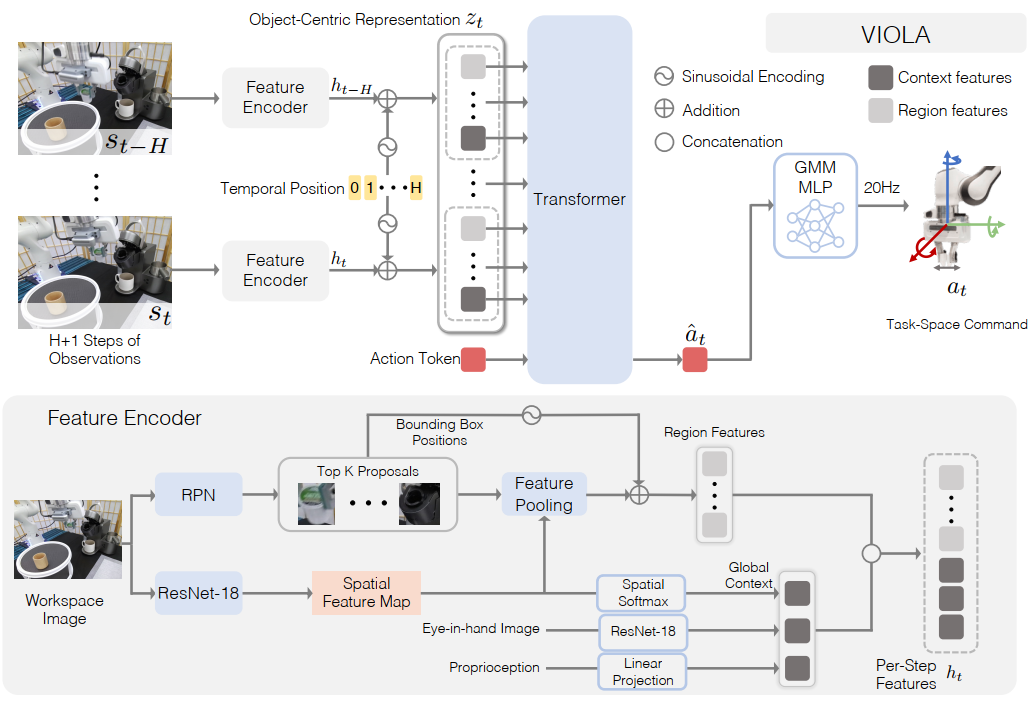
\includegraphics[width=0.7\textwidth]{figures/images/viola/viola_architecture.png}
        \caption{The VIOLA architecture proposed in \cite{zhu2023viola}. (Top) The overall control architecture is based on a Transformer module that processes a stack of \textit{per-step features} $h_{t}$, obtained from the Feature Encoder, to generate a final action embedding, which is then input into a GMM policy. (Bottom) The Feature Encoder builds both local and global features. Local features correspond to regions of interest extracted by the RPN. Global features are obtained by processing the workspace image, the image from the camera on the gripper, and proprioceptive information.
        }
    \label{fig:viola_architecture}
    
\end{figure}

\begin{figure}[t]
    \centering
    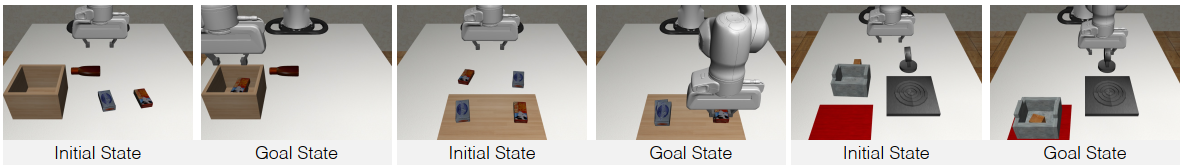
\includegraphics[width=0.9\textwidth]{figures/images/viola/viola_task.png}
    \caption{Simulation tasks on which the VIOLA \cite{zhu2023viola} method was tested. (Left) Sorting task. (Center) Stacking task. (Right) BUDS-Kitchen task}
    \label{fig:viola_task}
    
\end{figure}

This method was first evaluated in a simulation environment across three tasks, as depicted in Figure \ref{fig:viola_task}. Various testing scenarios were considered, including different object placements, the introduction of distractor objects, and changes in camera position. Generally speaking, VIOLA outperformed all baselines across these testing conditions, further demonstrating the utility of object priors in enhancing the robustness of such methods. However, similar to \cite{devin2018deep}, the testing scenarios were relatively simple, with clear distinctions between distractors and objects of interest. The distractors were objects never seen during the demonstration and were not involved in manipulation, making them relatively easy for the model to discriminate.

In the works discussed so far, the approach has primarily focused on leveraging object priors to directly predict the actions that the robot must perform. However, a different approach was proposed in \cite{belkhale2023plato}, where the authors introduced an alternative interpretation of object-centric concept. Instead of focusing on the robot perspective, they shifted the emphasis to the object perspective, proposing PLATO (Predicting Latent Affordances Through Object-Centric Play). PLATO is a learning framework that learns a \textbf{latent affordance space}, which describes how an object can be used (e.g., a block being grasped, a door knob being turned, or a drawer being opened).

The authors argue that learning these affordances (i.e., what happens to the object) rather than plans (i.e., what happens to the robot) from play leads to a simpler and more robust task representation that can operate over varying time horizons. This, in turn, results in more effective policies at test time. This paradigm shift allows the policy to reason about the environment more effectively: given access to an affordance (e.g., the door knob being turned) and a goal (e.g., an opened door), the policy can work backwards to infer the behavior needed to exploit that affordance (e.g., reaching the knob and rotating the gripper to turn it).

To reach this objective authors started from the observation that a single-object manipulation is composed of the following three phases:
\begin{enumerate}
    \item \textbf{Pre-interaction}, when the robot prepares to interact with an object (e.g., reaching for a block).
    \item \textbf{Interaction}, when the robot and the object engage in joint actions (e.g., pushing or pulling the block).
    \item \textbf{Post-interaction}, when the robot separates from the object, and the object may come to rest (e.g., the block stops moving).
\end{enumerate}
Given these three phases, the algorithm learns a \textbf{latent affordance distribution}. Specifically, the architecture comprises three learnable modules: \( E \), \( E' \), and \( \pi \). \( E \) models the posterior distribution, mapping the full interaction trajectory \( \tau^{i} \) to the corresponding latent affordance distribution, from which the affordance embedding \( z \) is sampled. \( E' \) is the prior module used during rollout. It takes the current state and the goal state as input and generates the affordance embedding \( z' \). This module is trained to match the posterior distribution modeled by \( E \). \( \pi \) represents the current policy, which generates the action \( a^{i} \) given the current state \( s^{i} \), the desired goal \( o_g \), and the latent embedding \( z \).

These three modules are trained end-to-end by minimizing the loss function in Formula \ref{eq:plato_equation}, which includes three terms. The first two terms correspond to the policy \( \pi \), ensuring it matches the ground-truth trajectories in the interaction and pre-interaction phases. The last term is the KL-divergence, used to train the posterior and prior modules \( E \) and \( E' \).

\begin{equation}
    \label{eq:plato_equation}
    \begin{aligned}
        \mathcal{L}_{PLATO} = -\log \left(\pi\left(a_{1: H}^{(i)} \mid s_{1: H}^{(i)}, o_g, z\right)\right)- \\ 
        \alpha \log \left(\pi\left(a_{1: H}^{(-)} \mid s_{1: H}^{(-)}, o_g, z\right)\right)+ \\ 
        \beta \operatorname{KL}\left(p(z) \| p\left(z^{\prime}\right)\right)
    \end{aligned}
\end{equation}
\begin{figure}[t]
    \centering
    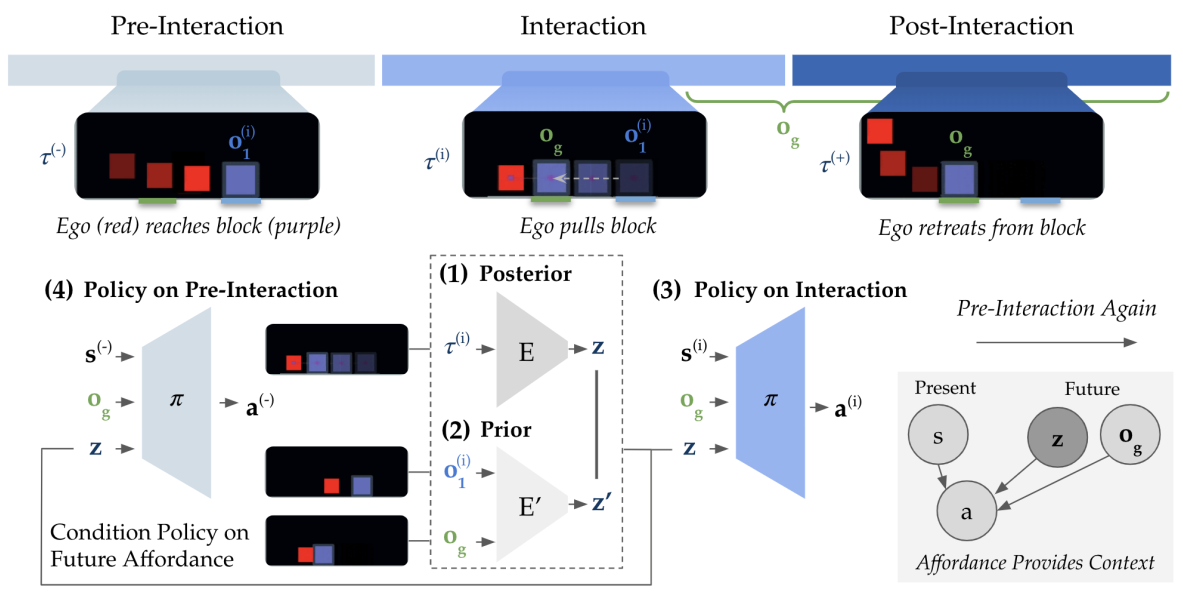
\includegraphics[width=0.7\textwidth]{figures/images/plato/plato.png}
    \caption{PLATO architecture proposed in \cite{belkhale2023plato}. The architecture is composed of different stages. (1) The posterior encoder \( E \) encodes the interaction sequence \( \tau^{(i)} \) into the affordance \( z \). (2) The prior encoder \( E' \) encodes the object initial state \( o^{(i)}_1 \) and goal state \( o_g \) to predict \( z \), with \( o_g \) sampled after the interaction. (3) The policy is trained to output actions during the interaction period conditioned on the affordance. Simultaneously, (4) it is trained to output actions during the pre-interaction period conditioned on the ``future" affordance.
    }
    \label{fig:plato}
    
\end{figure}

\begin{figure}[t]
    \centering
    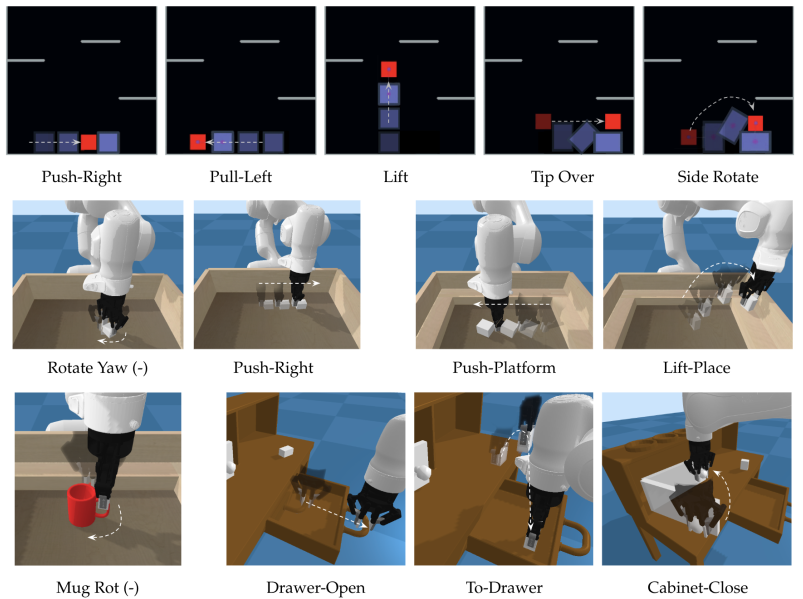
\includegraphics[width=0.7\textwidth]{figures/images/plato/tasks.png}
    \caption{ Testing scenarios and primitives proposed in \cite{belkhale2023plato}. (Top) \textbf{Block2D} Environment primitive examples. (Center) \textbf{Block3D} and \textbf{Block3DPlatform} primitive examples. (Bottom) The left image shows an example primitive in \textbf{Mug3D-Platforms}. The right three images show sample tasks from \textbf{Playroom3D}.}
    \label{fig:plato_task}
    
\end{figure}

Finally, this method was tested in a variety of scenarios, including both single-object and multiple-object manipulation with different manipulation primitives (Figure \ref{fig:plato_task}). However, in the multi-object scenarios, the system was only tested on single-object manipulation primitives.

This work is particularly noteworthy as it demonstrates that a policy can be learned by solving an inverse problem, starting from object affordances and deriving the corresponding robot trajectories. It also shows that the policy can be conditioned based on the desired goal state. However, certain aspects were not addressed in this work, such as the potential presence of distractor objects and tasks requiring the manipulation of multiple objects. Additionally, the affordances were learned in the object space (i.e., with known object poses) rather than in the high-level image space.


\paragraph{Discussion}
\subsubsection{Inverse Reinforcement Learning}
\label{sec:irl}
The \textit{Inverse Reinforcement Learning} (IRL) problem, also known as \textit{Inverse Optimal Control}, is a LfD algorithm that addresses a significant challenge in Reinforcement Learning: designing an appropriate reward function for a given problem.

In many manipulation problems \cite{kalashnikov2018scalable}, using a binary and sparse reward function, where the reward is 1 if the task is completed correctly and 0 otherwise, can result in very long and inefficient training periods. For instance, in a reaching problem where the goal is to simply reach an object, the agent would receive a reward of 0 most of the time. More critically, actions that bring the agent closer to the object and actions that move it farther away would yield the same reward. In this simple example, a better reward function would measure the relative distance between the agent and the object. While this information can be easily obtained in simulations, it is often unavailable in real-world settings, forcing algorithm designers to make assumptions such as having prior knowledge about the object's location.

To address this issue, several research approaches have been proposed. One prominent approach is \textit{Reward Shaping}. In this method, the goal is to make the reward function more informative by introducing intermediate rewards during the agent's experience. These intermediate rewards are hand-engineered and require some degree of \textit{domain knowledge}.

The second approach, which is the focus of this chapter, is Inverse Reinforcement Learning (IRL). In IRL, the main idea is to \textbf{learn} the reward function $R$ which explains the expert behaviors contained in the dataset $\mathcal{D}^{E}$, and then use the learned $R$ to train the agent using classic RL algorithms.

The IRL procedure was introduced in \cite{abbeel2004apprenticeship}, and it is described by Algorithm \ref{alg:irl}. Essentially, the IRL algorithm is an iterative process where the parametrized reward function $R_{\omega}$ is first updated according to a given objective function $\mathcal{L}$. Subsequently, the updated reward function is used to update the learner's policy $\pi_{\theta}^{L}$.

\begin{algorithm}
\caption{Classic feature matching IRL algorithm}
\label{alg:irl}
\begin{algorithmic}
\Require Dataset of expert trajectories $\mathcal{D} = \left \{ \boldsymbol{\tau}^{E}_{i} \right \}^{N}_{i=1}$ 
\Require Reward function $R_{\omega}$, policy $\pi^{L}_{\theta}$ 
\While {policy improves}
    \State Evaluate the state-action visitation frequency $\mu$ of the current policy $\pi^{L}_{\theta}$
    \State Evaluate the objective function $\mathcal{L}$, w.r.t. $\mu$ and the dataset $\mathcal{D}$
    \State Update the reward-function parameters $\omega$ based on $\mathcal{L}$
    \State Update the policy $\pi^{L}_{\theta}$ through an RL algorithm, using the updated $R_{\omega}$
\EndWhile
\end{algorithmic}
\end{algorithm}

Generally speaking, the IRL approach faces two main challenges:
\begin{itemize}
    \item The learning process can be time-consuming and impractical for high-dimensional problems due to the double-nested optimization procedure.
    \item The IRL problem is \textit{ill-posed} because multiple reward functions can produce the same set of actions.
\end{itemize}

Despite these practical and theoretical challenges, various significant scientific contributions have been made in this field.

To solve the problem of multiple solutions for the reward function, constraints have been added to the optimization problem. Specifically, based on the type of constraint, there are two approaches:
\begin{enumerate}[label=\textbf{(\alph*)}]
    \item The \textit{Maximum Margin Prediction} (MMP) approach \cite{ratliff2006maximum_margin,ratliff2009learning_to_search}.
    \item The \textit{Maximum Entropy} (Max-Ent) approach \cite{ziebart2008maximum_entropy,wulfmeier2015deep_inverse_rl,finn2016guided_cost_learning}.
\end{enumerate}

The \textit{MMP} methods assume that the demonstrated trajectories are \textbf{optimal} and operate in a \textbf{deterministic} setting. The aim is to find the cost function such that the reward of the demonstrated trajectories, $R(\boldsymbol{\tau}^{E})$, is greater than the reward of all alternative trajectories, $R_{\omega}(\boldsymbol{\tau})$, by a certain margin $m$, solving the optimization problem formalized in Formula \ref{eq:mmp}.
\begin{equation}
\label{eq:mmp}
\underset{\omega, m}{\max} \ m \quad \text{s.t.} \quad R_{\omega}(\boldsymbol{\tau}^{E}) \geq \max (R_{\omega}(\boldsymbol{\tau})) + m
\end{equation}
The main problem with this formulation is that it does not handle the case in which the expert behavior is sub-optimal, leading to an ambiguous notion of margin.

In the \textit{Max-Ent} approach, the goal is to find the reward function parameters $\psi$ that drive the policy to maximize the entropy, subject to feature expectation matching (Formula \ref{eq:max_ent}).
\begin{equation}
    \label{eq:max_ent}
     \underset{\psi}{\max} \ \mathcal{H}(\pi^{r_{\psi}}) \quad \text{s.t.} \quad \mathbb{E}_{\pi^{r_{\psi}}}[\mathbf{f}] = \mathbb{E}_{\pi^{*}}[\mathbf{f}]
\end{equation}
The Max-Ent approach is the most popular in the IRL field since it removes the ambiguous aspects of the previous formulation. In the original work, the reward function was a linear combination of the features, i.e., $r_{\psi} = \psi^T \mathbf{f}$. However, this reward formulation is not suited for high-dimensional feature spaces, which may require the capability to model non-linear reward structures. In \cite{wulfmeier2015deep_inverse_rl}, a deep neural network was used to model the reward function. In this work, the neural network maps the feature vector $\mathbf{f}$ to the reward value and is trained according to the Maximum-Entropy setting. Experimental results have shown that the ability to approximate highly non-linear reward functions is essential for successfully solving tasks in high-dimensional discrete state spaces. A generalization to continuous state spaces was proposed in \cite{finn2016guided_cost_learning}. 

In particular, \cite{finn2016guided_cost_learning} addressed the problem of learning a cost function in a high-dimensional continuous state space with \textbf{unknown dynamics}. Starting from the exponential trajectory distribution $p(\tau) = \frac{1}{Z} \exp(-c_{\theta}(\tau))$,
the main difficulty is the estimation of the partition function $Z$, needed to compute the negative log-likelihood loss function (Formula \ref{eq:loss_reward_guided_cost_learning}).
\begin{equation}
    \label{eq:loss_reward_guided_cost_learning}
    \mathcal{L}_{\theta} = \frac{1}{N} \sum_{\tau^{E}_{i} \in D_{demo}} c_{\theta}(\tau^{E}_{i}) + \log(Z)
\end{equation}
Since the dynamics are unknown, the idea was to estimate the partition function through the trajectories obtained from the current policy rollouts, with the hypothesis that, during the learning of the cost function, the current policy drives the distribution towards regions where samples are more useful.

\begin{algorithm}[htbp]
\caption{Guided-Cost-Learning Algorithm \cite{finn2016guided_cost_learning}}
\label{alg:guided_cost_learning}
\begin{algorithmic}
\REQUIRE Initial controller $q_{k}(\tau)$ 
\FOR {i = 1, \dots, N}
    \STATE Generate $D_{traj}$ from $q_{k}(\tau)$
    \STATE $\mathcal{D}_{samp} \leftarrow \mathcal{D}_{samp} \bigcup \mathcal{D}_{traj}$
    \STATE Update the cost-function parameters, using $\mathcal{D}_{samp}$ and $\nabla_{\theta}\mathcal{L(\theta)}$
    \STATE Update the controller $q_{k+1}(\tau) \leftarrow q_{k}(\tau)$ according to \cite{levine2014lqr_flm} and using $\mathcal{D}_{traj}$
\ENDFOR
\end{algorithmic}
\end{algorithm}

Starting from these considerations, Algorithm \ref{alg:guided_cost_learning} was proposed. The algorithm returns a \textit{Linear-Quadratic Gaussian} \cite{levine2014lqr_flm} controller $q_{k}$, obtained by solving the problem in Formula \ref{eq:lqgc}.
\begin{equation}
    \label{eq:lqgc}
    \begin{aligned}
    q_{k} = \underset{q}{\arg \min} \ \mathbb{E}[c_{\theta}(\tau)] - \mathcal{H}(\tau) \quad \\ \text{s.t.} \quad p(s_{t+1}|s_{t},a_{t}) = \mathcal{N}(s_{t+1}; f_{x_t}x_{t}+f_{u_t}u_{t}, F_{t})
    \end{aligned}
\end{equation}

The cost function was parameterized according to a neural network, and experiments performed on real-robot manipulation tasks such as dish placement and pouring proved the effectiveness of the proposed method and the necessity of a non-linear representation of the cost function for complex problems, outperforming the classic Max-Ent method.

Recent methods have aimed to advance IRL towards more complex learning scenarios, such as learning a reward function from video demonstrations. In \cite{das2021model_based_irl_from_vd}, the architecture shown in Figure \ref{fig:model_based_irl} was proposed. The goal was to obtain the parameters $\Psi$ of a cost function $C_{\Psi}(\hat{\boldsymbol{\tau}}, z_{goal})$, enabling the derivation of a sequence of actions by minimizing the cost function itself (Formula \ref{eq:das2021model_based_irl_from_vd}).
\begin{equation}
\label{eq:das2021model_based_irl_from_vd}
\textbf{a}_{new} = \textbf{a} - \eta \nabla_{a} C_{\Psi}(\hat{\boldsymbol{\tau}}, z_{goal}).
\end{equation}
Different cost functions were proposed, all aiming to reduce the distance between the current predicted keypoints and the goal keypoint configuration. The trajectory $\hat{\boldsymbol{\tau}}$ is a sequence of predicted states $[\hat{s}_{1}, \dots, \hat{s}_{T}]$, resulting from a learned dynamic model, $\hat{s}_{t+1} = f_{dyn}(\hat{s}_{t}, a_{t})$. 

Experimental results demonstrated that it is possible to learn a cost function from human/robot video demonstrations. However, the proposed setting was tested on a very simple reaching task, highlighting that much work remains to be done to establish the effectiveness or ineffectiveness of IRL in complex real-robot manipulation tasks starting from video demonstrations.

\begin{figure}[th]
    \centering
    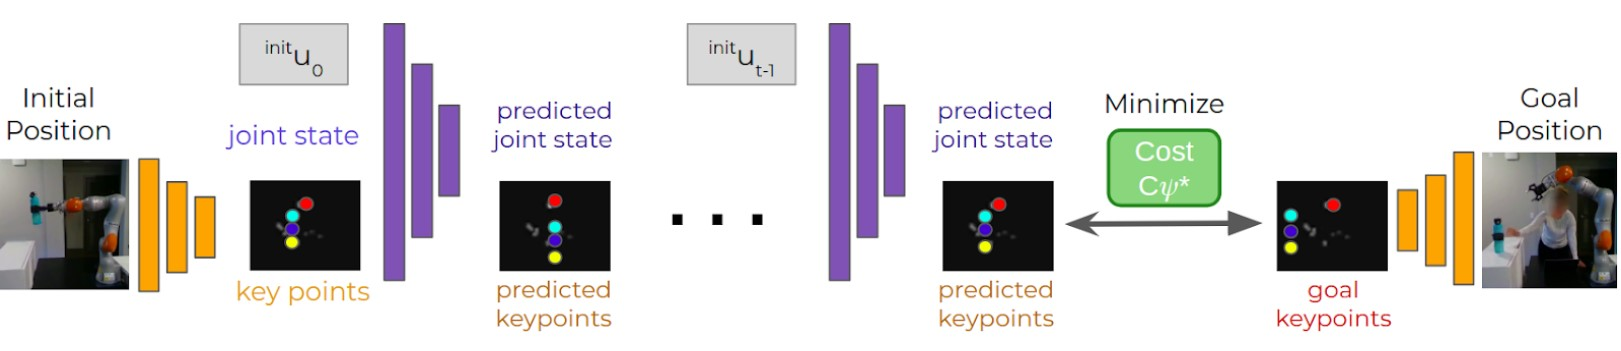
\includegraphics[width=\textwidth]{figures/images/model_based_irl/model_based_irl.jpg}
    \caption{Architecture proposed in~\cite{das2021model_based_irl_from_vd}.}
    \label{fig:model_based_irl}
\end{figure}

\subsubsection{Generative Adversarial Imitation Learning}
\label{sec:gail}
This section will be dedicated to the introduction of the \textit{Generative Adversarial Imitation Learning} (GAIL) approach. 

\subsubsection{Learning from Observation}

\begin{figure}[t]
    
    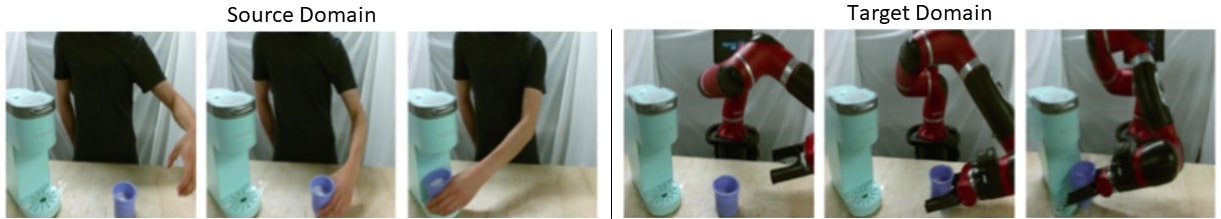
\includegraphics[width=\textwidth]{figures/images/embodiment_mismatch/embo.jpg}
    \caption{Representation of \textbf{embodiment mismatch problem}. (Left) The source domain
    represented by a video of human performing a task. (Right) The target domain, represented
    by the robot that executes the observed task.}
    \label{fig:embo_mismatch}
    
\end{figure}

\label{sec:lfo}
In the previous sections, the methodologies assumed access to the agent actions, working with state-action trajectories. In \textit{Learning from Observation} (LfO), this assumption is relaxed, and methods for learning from \textbf{state-only} demonstrations are introduced. This approach has gained significant attention in recent years~\cite{torabi2019recent_advances_lfo} because it theoretically enables a robotic system to be programmed as naturally as possible. Ideally, a robotic system should be able to replicate a task by observing a human or another robot performing it, without access to the actions taken, in contrast to the methods described thus far.

To address this problem, several questions need to be answered:

\begin{enumerate}
\item How can embodiment mismatches be resolved when the demonstrator has a different embodiment than the imitator?
\item How can the correspondence problem be handled when the demonstrator viewpoint differs from the imitator?
\item Once the perception subsystem issues are resolved, how is the policy $\pi^{L}$ obtained?
\end{enumerate}

The first question refers to the \textit{correspondence problem} introduced in Section~\ref{sec:sod}. This problem arises when the demonstrator embodiment differs from that of the learner, meaning that methods cannot directly use the recorded trajectories of the demonstrator.

One approach to solving this problem is to use methods that perform \textit{image-to-image} translation. This involves using generative deep architectures to transform images of a subject in one domain (e.g., a human demonstrator) into images where the context remains the same, but the subject is different (e.g., the human demonstrator is replaced by the target robot) as depicted in Figure \ref{fig:embo_mismatch}. This approach has been followed by authors in \cite{smith2019avid,xiong2021learning_by_watching,li2021meta_watching_video_demonstration}.

Specifically, the authors in \cite{smith2019avid, xiong2021learning_by_watching} used the Cycle-GAN architecture \cite{zhu2017cycle_gan} to translate images from the source domain (human images) to the target domain (robot images) in an unsupervised manner. The work in \cite{zhu2017cycle_gan} shifted the translation problem from a paired image setting, where each source domain image has a corresponding target domain image, to an unpaired image setting, where the source domain image does not have a corresponding target domain image.

To address this, Cycle-GAN introduces a novel learning procedure involving two translation models: $G: X \rightarrow Y$ and $F: Y \rightarrow X$. The first model maps inputs from the source domain to the target domain, while the second model maps inputs from the target domain back to the source domain. These two models are trained in an adversarial setting by minimizing the loss function shown in Formula \ref{eq:cycle_gan_loss}.
\begin{equation}
    \label{eq:cycle_gan_loss}
    \begin{aligned}
        \mathcal{L}(G,F,D_X,D_Y) &= \mathcal{L}_{GAN}(G,D_Y,X,Y) + \\
        &\quad \mathcal{L}_{GAN}(F,D_X,Y,X) + \lambda\mathcal{L}_{cyc}(G,F) 
        \\ \\
        \mathcal{L}_{GAN}(Z,D_{K},S,T) &= \mathbb{E}_{t \sim p_{data}(t)}\left[ \log(D_K(t)) \right] + \\
        &\quad \mathbb{E}_{s \sim p_{data}(s)}\left[ \log(1 - D_K(Z(s))) \right]    
        \\ \\
        \mathcal{L}_{cyc}(G,F) &= \mathbb{E}_{x \sim p_{data}(x)}\left[ \|F(G(x)) - x\|_{1} \right] +  \\
        &\quad \mathbb{E}_{y \sim p_{data}(y)}\left[ \|G(F(y)) - y\|_{1} \right]
        \end{aligned}
\end{equation}

Here, $\mathcal{L}_{GAN}$ is the adversarial loss component, where the discriminator $D_{K}$ is trained to distinguish between real samples $t \in T$ and translated samples $Z(s)$. The generator $Z$ is trained to generate samples that are as similar as possible to those in the target domain, starting from samples in the source domain. Meanwhile, $\mathcal{L}_{cyc}$ is a loss term that aims to maintain consistency between the generated samples and the ground truth one.

The application of this concept in the domain of interest, lead to a dataset for the source domain was composed of human demonstrations as well as a small amount of ``random" data, in which the human moves around the scene but does not specifically attempt the task, while for the target domain, it consists of robot images executing randomly sampled actions in a few different settings.

The second question also addresses a variant of the correspondence problem, where, in addition to the embodiment mismatch, the problem of \textit{different viewpoints} is also encountered (Figure \ref{fig:time_contrastive}). This issue has been tackled in \cite{sermanet2018time_contrastive, liu2018imitation_from_observation}.

In \cite{sermanet2018time_contrastive}, a Convolutional Neural Network was trained using a \textit{Triplet-Loss} \cite{schroff2015triplet_loss}. The aim was to train a network to predict an embedding independent of the viewpoint, but containing only task-relevant features. To achieve this, the network had to produce an embedding, $f(x)$, such that $|| f(x^{a}_{i}) - f(x^{p}_{i})||^{2}_{2} + \alpha < || f(x^{a}_{i}) - f(x^{n}_{i})||^{2}_{2}$ for all $(f(x^{a}_{i}), f(x^{p}_{i}), f(x^{n}_{i})) \in \mathcal{T}$, where $\mathcal{T}$ is the set of all possible triplets in the dataset. This implies that embeddings produced by samples from different viewpoints, but sharing the same time-step, $(x^{a}_{i},x^{p}_{i})$, should be similar, while embeddings produced by samples from the same viewpoint, but at different time-steps, $(x^{a}_{i},x^{n}_{i})$, should be different (Figure \ref{fig:time_contrastive}).

In \cite{liu2018imitation_from_observation}, a different approach was employed. Here, a \textit{context translation problem} was addressed using an Encoder-Decoder architecture (Figure \ref{fig:context-translation}). The proposed architecture was trained on pairs of demonstrations, $\mathcal{D}_{i}=[o^{i}_{0},o^{i}_{1},\dots,o^{i}_{T}]$ and $\mathcal{D}_{j}=[o^{j}_{0},o^{j}_{1},\dots,o^{j}_{T}]$, composed of visual observations. Samples in $\mathcal{D}_{i}$ come from the source context $\omega_{i}$, while samples in $\mathcal{D}_{j}$ come from the target context $\omega_{j}$. The model must output the observations in $\mathcal{D}_{j}$ conditioned on both $\mathcal{D}_{i}$ and the first observation $o^{j}_{0}$ from the target domain.

As will be explained next, the outputs of both the Time-Contrastive and the Context-Translation networks can be used to obtain an engineered reward function.

\begin{figure}[t]
    \centering
    \begin{subfigure}[b]{0.50\textwidth}
        \centering
        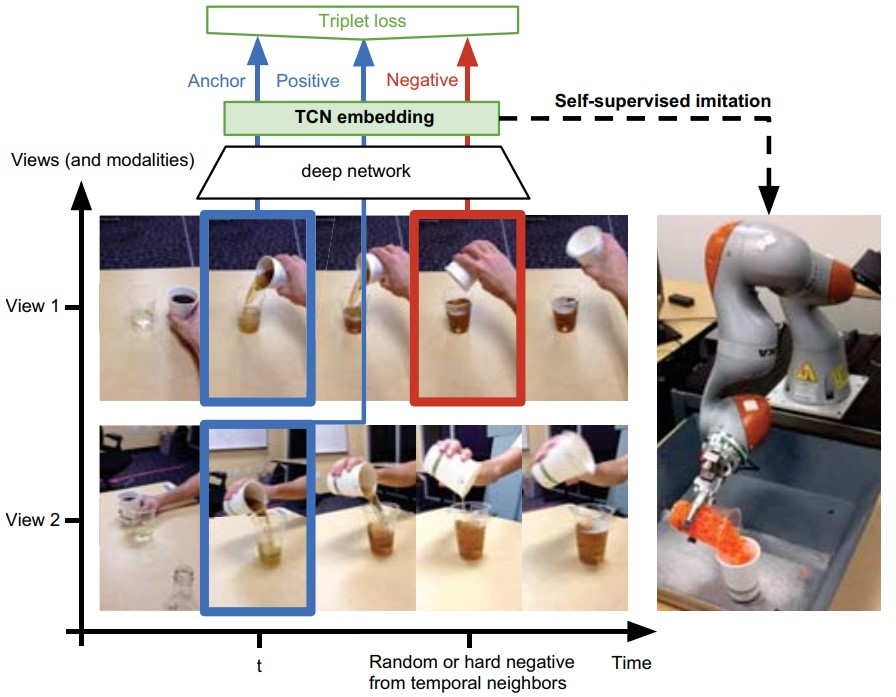
\includegraphics[width=\textwidth]{figures/images/view_point_mismatch/time-contrastive-network.jpg}
        \caption{\textit{Time-Contrastive network}, proposed in~\cite{sermanet2018time_contrastive}.}
        \label{fig:time_contrastive}
    \end{subfigure}
    \hfill
    \begin{subfigure}[b]{0.45\textwidth}
        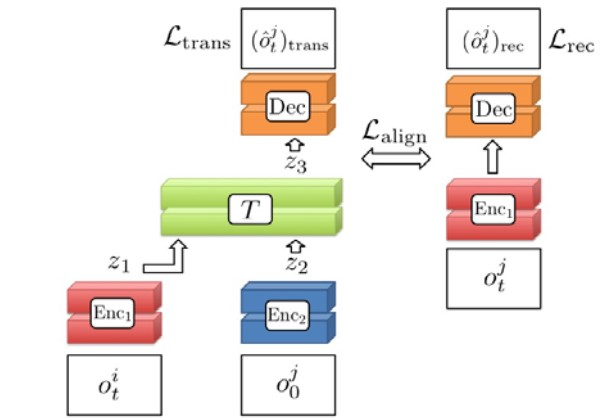
\includegraphics[width=\textwidth]{figures/images/view_point_mismatch/context-translation-model.jpg}
        \caption{\textit{Context-Translation network}, proposed in~\cite{liu2018imitation_from_observation}}
        \label{fig:context-translation}
    \end{subfigure}
    \caption{Examples of how the mismatch between demonstrator viewpoint and learner viewpoint can be handled.}
    \label{fig:differet_viewpoint}
\end{figure}


The third question concerns the method by which the final learned policy is derived. To present the different approaches, it is essential to distinguish between \textit{Model-Free} and \textit{Model-Based} methods (Figure \ref{fig:lfo_taxonomy}).

\begin{figure}[t]
    
    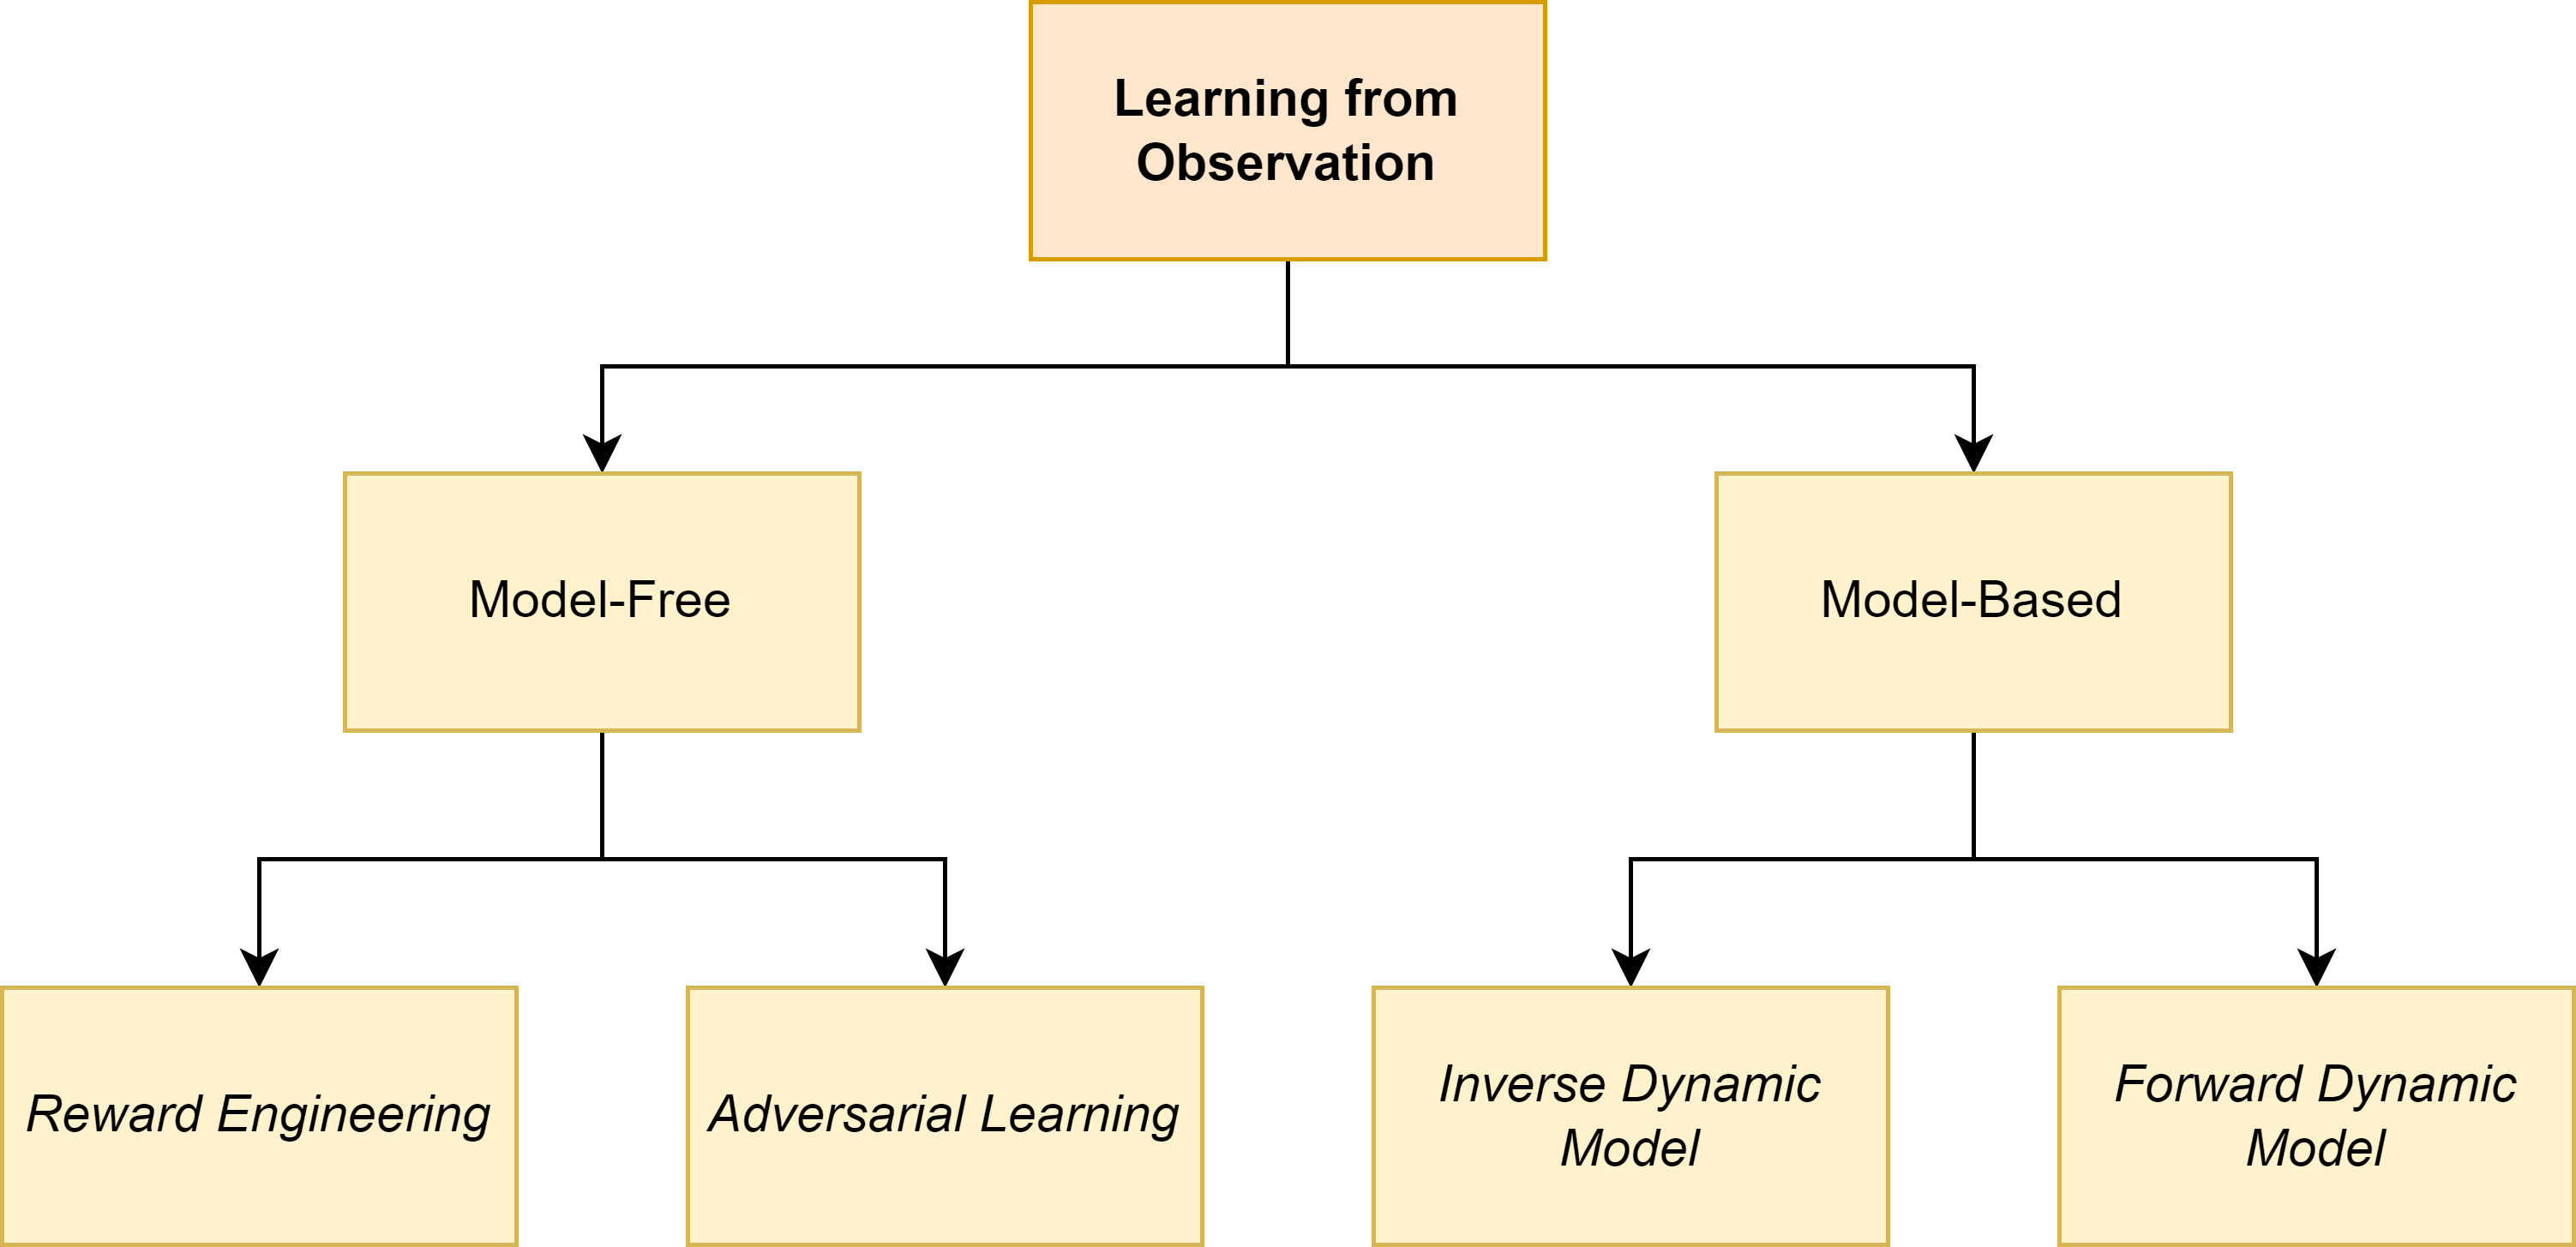
\includegraphics[width=0.8\textwidth]{figures/images/lfo_taxonomy.png}
    \caption{Learning from Observation taxonomy}
    \label{fig:lfo_taxonomy}
    
\end{figure}


\paragraph*{Model-Free}\mbox{}\\
Model-Free methods are characterized by the fact that they do not leverage knowledge about the environment dynamics, which can either be given a priori or learned through data-driven approaches. A further classification must be done between \textit{Reward Engineering} and \textit{Adversarial Learning} approaches.

\textbf{Reward Engineering} methods are characterized by the use of a hand-designed reward function to train the policy according to the Reinforcement Learning paradigm \cite{sutton2018reinforcement}. Methods based on this approach include \cite{liu2018imitation_from_observation,sermanet2018time_contrastive,xiong2021learning_by_watching,zakka2022xirl}.

In \cite{liu2018imitation_from_observation}, the reward function is defined as in Formula \ref{eq:liu2018imitation_from_observation_reward}.
\begin{equation}
    \label{eq:liu2018imitation_from_observation_reward}
    \begin{aligned}
        R(o^{l}_{t}) = -\left\|Enc_{1}(o^{l}_{t}) - \frac{1}{n} \sum_{i=1}^{n}F(o_{t}^{i},o_{0}^{l})\right\|^{2}_{2} - \\ w_{rec} \left\|o^{l}_{t} - \frac{1}{n} \sum_{i=1}^{n}M(o_{t}^{i},o_{0}^{l})\right\|^{2}_{2}
    \end{aligned}
\end{equation}
The first term is the classic Feature Tracking reward function, which aims to minimize the Euclidean Distance between the encoding of the current learner observation $o^{l}_{t}$ and the encoding of the demonstration in the learner context. The second term penalizes the policy for experiencing observations that differ from the translated observation.

In \cite{sermanet2018time_contrastive}, the reward function is defined according to Formula \ref{eq:sermanet2018time_contrastive_reward}.
\begin{equation}
    \label{eq:sermanet2018time_contrastive_reward}
    \begin{aligned}
        R(\textbf{v}_{t}, \textbf{w}_{t}) = - \alpha \left\| \textbf{w}_{t} - \textbf{v}_{t} \right\|^{2}_{2} - \beta \sqrt{\gamma + \left\| \textbf{w}_{t} - \textbf{v}_{t} \right\|^{2}_{2}}
    \end{aligned}
\end{equation}
Where $\textbf{v}_{t}$ is the TCN embedding of the video demonstration at timestep $t$, and $\textbf{w}_{t}$ is the TCN embedding produced by the robot observation (Figure \ref{fig:time_contrastive}).

In \cite{xiong2021learning_by_watching}, a \textbf{keypoint-representation} (Figure \ref{fig:lbw}) is obtained for both the current robot observations $z_{t}$ and each frame of the translated demonstration video $\{z^{E}_{p}\}_{p=1}^{T}$. The reward is then computed as in Formula \ref{eq:xiong2021learning_by_watching_reward}.
\begin{equation}
    \label{eq:xiong2021learning_by_watching_reward}
    \begin{aligned}
        R(z_{t},z_{t+1},z^{E}) = - \lambda_{1} \min_{p} \left\|z_{t}-z^{E}_{p}\right\| - \\ \lambda_{2} \min_{p} \left\|(z_{t+1}-z_{t}) - (z^{E}_{p+1}-z^{E}_{p})\right\|
    \end{aligned}
\end{equation}
The main idea is to generate actions that minimize the distance between the translated keypoints and the keypoints obtained from the current robot observation, thereby reproducing the demonstrated trajectory. The \textit{min} operator is necessary because the robot and the demonstration are not temporally aligned; there is no a priori knowledge about which demonstration frame corresponds to the current agent state.

\begin{figure}[t]
    \centering
    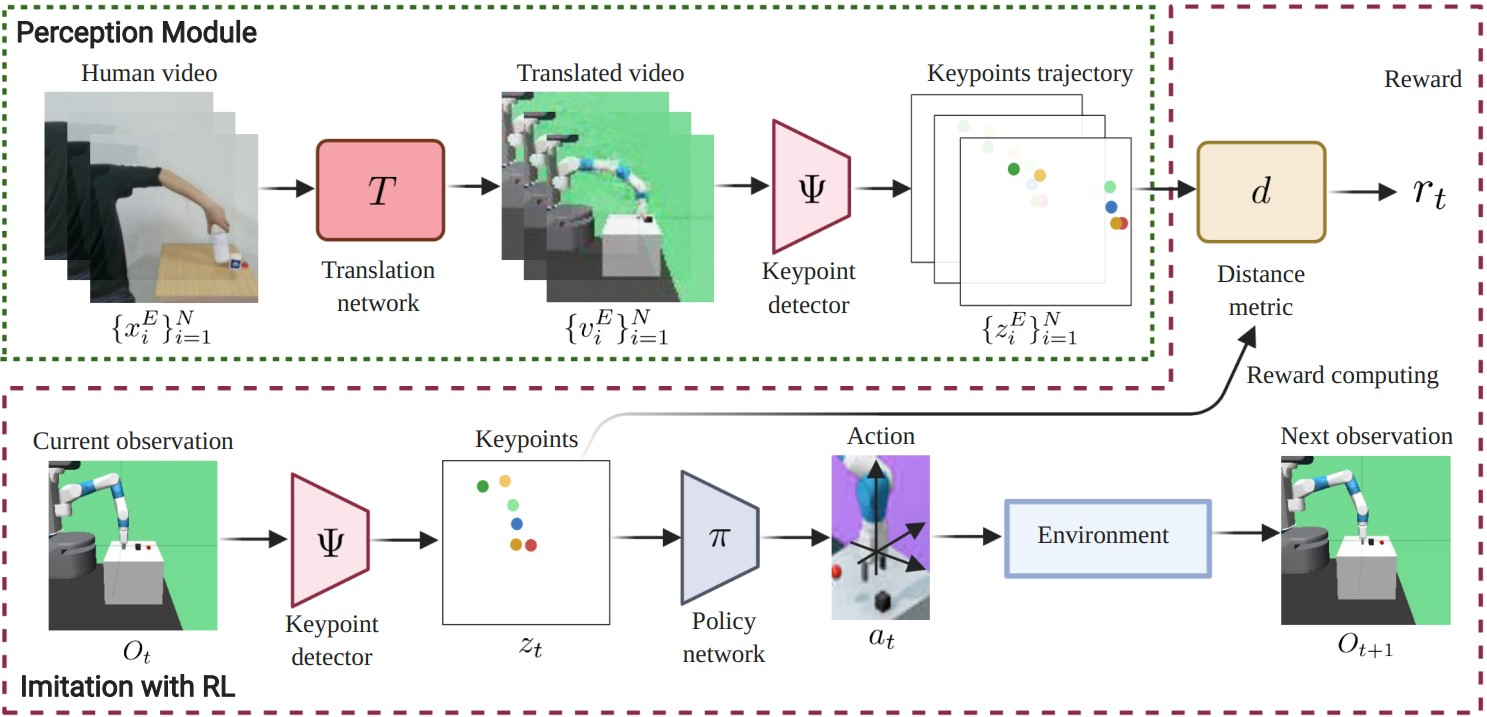
\includegraphics[width=0.8\textwidth]{figures/images/learning_by_watching/learning_by_watching.jpg}
    \caption{Architecture proposed by~\cite{xiong2021learning_by_watching}.}
    \label{fig:lbw}
\end{figure}

In \cite{zakka2022xirl}, the reward function was defined as $R(s_{t}) = -\frac{1}{k} \ || \phi(s_{t}) - g||^{2}_{2}$, where $g$ is the goal embedding, defined as the mean embedding of the last frame of all the demonstration videos in the dataset, while $\phi(s_{t})$ is the embedding of the current observation. Experimental results, on simulation data proved that the proposed method can be used to learn tasks from cross-embodiment demonstrations, outperforming baseline \cite{sermanet2018time_contrastive} in terms of both sample efficiency and performance.


\paragraph*{Adversarial Learning} methods rely on the Adversarial Learning paradigm and are closely related to the GAIL methods (Section \ref{sec:gail}). Unlike the methods discussed in the GAIL section, these methods do not assume access to the demonstrator's actions. Preliminary works in this area have been proposed in \cite{merel2017learning,torabi2018gaifo}.

The goal of authors in \cite{merel2017learning} was to demonstrate that the Adversarial Learning setting can be effectively used even without action information. To test this hypothesis, the authors conducted a series of experiments in simulation for a walking task, where the same RL policy was trained in two contexts: one where the Discriminator had access to the (state, action) pair, and another where the Discriminator had access to state-only demonstrations. The results showed no substantial difference between the two settings, supporting the hypothesis that the essential information for task learning is contained in the state.

\begin{algorithm}[t]
\caption{GAIfO algorithm \cite{torabi2018gaifo}}
\label{alg:gaifo_algorithm}
\begin{algorithmic}
\REQUIRE Initial policy $\pi^{L}_{\phi}$, Initial Discriminator $D_{\theta}$
\REQUIRE State-only expert demonstration trajectories $\tau^{E} = \left \{ (s,s') \right \}$
\WHILE {Policy Improves}
    \STATE Execute $\pi^{L}_{\phi}$ and collect state transitions $\tau^{L} = \left \{ (s,s') \right \}$
    \STATE Update $D_{\theta}$, with $\mathcal{L}_{D_{\theta}} = - \ ( \ \mathbb{E}_{\tau^{L}}[\log (D_{\theta}(s, s')) ] + \mathbb{E}_{\tau^{E}}[\log(1 - D_{\theta}(s, s'))] \ )$
    \STATE Update $\pi^{L}_{\phi}$, with reward $ r_{\pi^{L}_{\phi}} = - \ ( \ \mathbb{E}_{\tau^{L}}[\log(D_{\theta}(s, s'))] \ )$
\ENDWHILE
\end{algorithmic}
\end{algorithm}

The next significant work was proposed by the authors of \cite{torabi2018gaifo}, who formalized the \textit{GAIfO} algorithm (Algorithm \ref{alg:gaifo_algorithm}), an extension of GAIL \cite{ho2016gail} to state-only demonstrations. The proposed algorithm was used to train a network to solve tasks in a simulation environment \cite{brockman2016openai}, with both low-dimensional state representation and visual-state representation. Results regarding the number of demonstrated trajectories are reported in Figure \ref{fig:gaifo_results}.

As noted from the results, GAIfO outperforms previous observation-based methods \cite{sermanet2018time_contrastive,torabi2018bco} in settings with a low number of expert trajectories. The main drawback of GAIfO is the \textbf{high number of environmental interactions} needed to learn a policy, as it uses the model-free TRPO \cite{schulman2015trpo} algorithm. This issue was addressed by DEALIO \cite{torabi2021dealio}, which replaced the model-free algorithm with PILQR \cite{chebotar2017pilqr}, a model-based RL algorithm discussed next.

\begin{figure}[tb]
     \centering
     \begin{subfigure}[b]{0.8\textwidth}
        \centering
         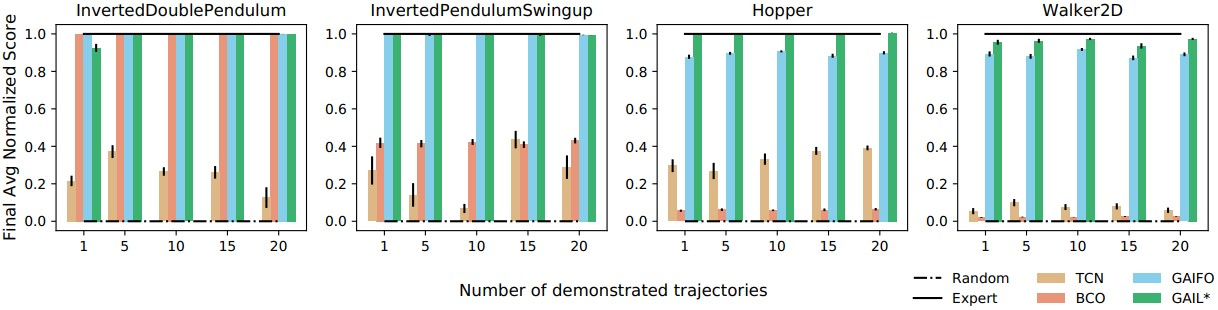
\includegraphics[width=\textwidth]{Figures/images/gaifo_results/gaifo_results.jpg}
         \caption{Experimental results in low-dimensional state space}
         \label{fig:low_dimensional}
     \end{subfigure}
     \vfill
     \begin{subfigure}[b]{0.8\textwidth}
        \centering
         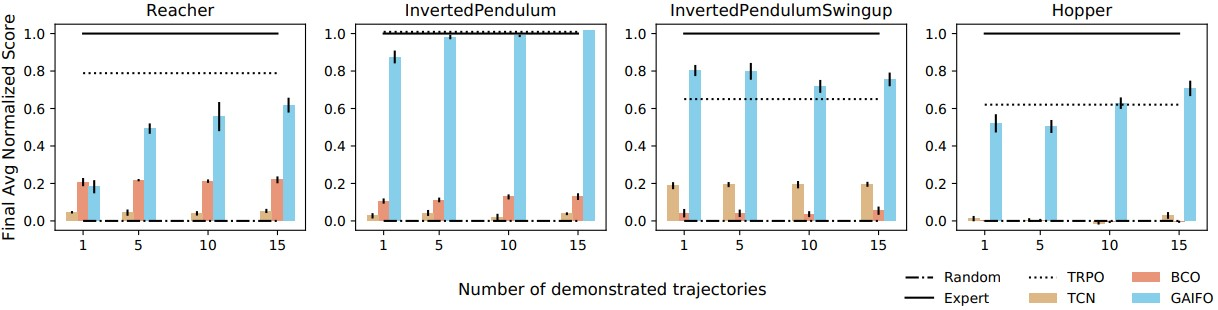
\includegraphics[width=\textwidth]{Figures/images/gaifo_results/gaifo_results_visual.jpg}
         \caption{Experimental results in high-dimensional state space}
         \label{fig:high_dimensional}
     \end{subfigure}
    \hfill
    \caption{Experimental results reported in \cite{torabi2018gaifo}.}
    \label{fig:gaifo_results}
\end{figure}



\paragraph*{Model-Based}\mbox{}\\
Model-Based methods leverage knowledge about the environment dynamics, which is learned through data-driven approaches. These methods can be further classified into \textit{Inverse Dynamic Model} and \textit{Forward Dynamic Model} approaches. 

The \textit{Inverse Dynamic Model} approach, given a transition $(s_{t}, s_{t+1})$, obtains a function $M$ that maps state transitions to actions, i.e., $a_{t} = M(s_{t}, s_{t+1})$. In contrast, the \textit{Forward Dynamic Model} approach, given a state-action pair $(s_{t}, a_{t})$, aims to learn a function $F$ that generates the next state $s_{t+1}$, i.e., $s_{t+1} = F(s_{t}, a_{t})$.

\textbf{Inverse Dynamic Model} methods include \cite{nair2017combining,torabi2018bco,guo2019hybrid_rl,radosavovic2021state_only_demo}.

In \cite{nair2017combining}, the goal was to develop a system capable of tying a knot in a rope. A self-supervised learning approach was used to train a Convolutional Neural Network. Given a pair of images $(I_{t}, I_{t+1})$ representing two successive rope states, the network was able to determine the action required to transition from state $I_{t}$ to state $I_{t+1}$. The network was trained using a dataset of 30K tuples $(I_{t}, a_{t}, I_{t+1})$ collected via an exploratory policy.

Authors in \cite{torabi2018bco} proposed a general approach, depicted in Figure \ref{fig:bco}, composed of two main parts: the learned Inverse Dynamic Model, $M_{\theta}$, and the learned policy $\pi_{\phi}$. The learning procedure is iterative. The model $M_{\theta}^{i}$ is updated by maximizing the probability $p_{\theta}(a_{t}|s_{t}, s_{t+1})$, using tuples $(s_{t}, a_{t}, s_{t+1})$ collected by the current policy. Once the dynamic model is updated, it infers the action $\tilde{a}_{t}$ given the demonstrations. The policy, having access to both state and action information, is then trained using classic Behavioral Cloning (BC) by optimizing the policy parameters through maximum-likelihood estimation $\phi^{*} = \underset{\phi}{argmax} \prod_{i=0}^{N} \pi^{L}_{\phi}(\tilde{a}_{i}|s_{i})$.

In \cite{guo2019hybrid_rl}, a similar approach to \cite{torabi2018bco} was used, but the agent's policy was trained using a combination of Behavioral Cloning and the Advantage Actor Critic (A2C) objective function \cite{mnih2016a2c} (Formula \ref{eq:a2c_reward}).
\begin{equation}
    \label{eq:a2c_reward}
    \begin{aligned}
        \mathcal{L}^{hyb}_{\theta} = \mathbb{E}_{s,a} \left[ A(s)\log(a|s;\theta) + \alpha \ \mathcal{H}(\pi^{L}(.|s)) \right] 
        + \\ \mathbb{E}_{(\hat{s}_{t}, \hat{s}_{t+1}) \sim D} \left[ \log(\pi^{L}(M(\hat{s}_{t}, \hat{s}_{t+1})|\theta)) \right].
    \end{aligned}
  \end{equation}
The main drawback is the assumption of access to the reward function, which can limit its applicability in real-robot manipulation tasks.

In \cite{radosavovic2021state_only_demo}, the work in \cite{Rajeswaran18_learning_complex_dexterous} was extended to state-only demonstrations, and the \textit{State-Only Imitation Learning} (SOIL) algorithm was proposed. This method addresses complex dexterous manipulation tasks, such as object reallocation, tool use, in-hand manipulation, and door opening, using a simulated humanoid hand. A neural network representing the Inverse Dynamic Model was trained by minimizing the L2-loss, given the action performed during the policy rollout. The policy was then updated according to the \textit{Demo Augmented Policy Gradient} (DAPG) method \cite{Rajeswaran18_learning_complex_dexterous}, adapted for state-only demonstrations, which follows the gradient updates described by Formula \ref{eq:dapg_updates}.
\begin{equation}
    \label{eq:dapg_updates}
    \begin{aligned}
        g_{SOIL} = g + \lambda_{0} \ \lambda_{1}^{k} \ \sum_{(s_{t}, \tilde{a}_{t}) \in D'} \nabla_{\theta}\log\pi^{L}_{\theta}(\tilde{a}_{t}, s_{t}),
    \end{aligned}
  \end{equation}

where $g$ is the Natural Policy Gradient term. The idea is to leverage the demonstrations at the beginning of the training and then exploit the RL algorithm to improve the behavior. Experiments performed in simulation showed that, compared to pure RL, the proposed method converges faster and produces more human-like behaviors.

\begin{figure}[tb]
    \centering
    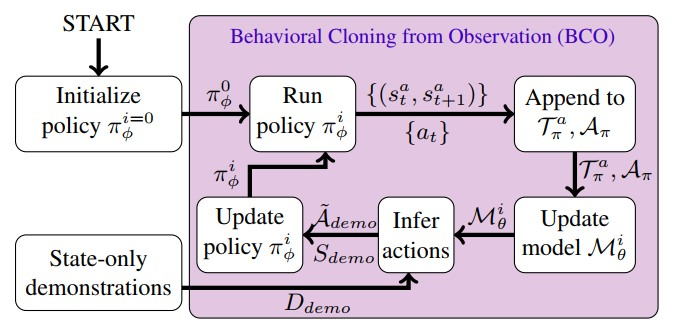
\includegraphics[width=0.6\textwidth]{figures/images/bco/bco.jpg}
    \caption{Representation of the learning procedure proposed by~\cite{torabi2018bco}}
    \label{fig:bco}
\end{figure}


\textbf{Forward Dynamic Model} methods include \cite{smith2019avid,torabi2021dealio}.

In \cite{smith2019avid}, once the human video demonstration was translated into the corresponding robot video, the policy was learned to use the model-based RL algorithm SOLARIS \cite{zhang2019solar}. This algorithm optimizes a controller using the Linear-Quadratic Regulator (LQR) procedure. The policy optimization occurs in a low-dimensional, highly regularized \textit{latent space}, generated using Variational Inference \cite{Kingma2014_vae}. Starting from a sequence of observations and actions, a Global Dynamic Model over the latent trajectory is obtained. Then, given the Latent Dynamic Model, a Linear-Gaussian Controller is derived using LQR-FLM \cite{levine2014lqr_flm}. Real-world robotic experiments demonstrated that with just \textbf{2 hours} of robot interaction, it was possible to outperform previous works such as \cite{sermanet2018time_contrastive,torabi2018bco} and classic BC algorithms in tasks like "coffee making" (Figure \ref{fig:embo_mismatch}) and cup-retrieving, where the robot retrieves a cup from a closed drawer.

In \cite{torabi2021dealio}, the sample inefficiency problem of GAIfO \cite{torabi2018gaifo} was addressed. The approach combined the adversarial learning setting with state-only demonstrations, which had shown promising results (Figure \ref{fig:gaifo_results}), with a more data-efficient RL algorithm like PILQR \cite{chebotar2017pilqr}. PILQR's core is the LQR optimization procedure. Generally, it returns a \textit{linear-gaussian controller} (Formula \ref{formula:linear_gaussian_controller}) that optimizes a \textit{quadratic-cost function} (Formula \ref{formula:quadratic_cost_function}) under the assumption of \textit{linear-gaussian dynamics} (Formula \ref{formula:gaussian_dyn}).

\begin{equation}
\label{formula:linear_gaussian_controller}
    \pi(a_{t}|s_{t}) = \mathcal{N}(K_{t}s_{t} + k_{t}, S_{t})
\end{equation}

\begin{equation}
\label{formula:quadratic_cost_function}
c(s_{t},a_{t}) = \begin{bmatrix}
s_{t}
\\ 
a_{t}
\end{bmatrix}^{T}C_{t}\begin{bmatrix}
s_{t}
\\ 
a_{t}
\end{bmatrix} + \begin{bmatrix}
s_{t}
\\ 
a_{t}
\end{bmatrix}^{T} c_{t} + cc_{t}
\end{equation}

\begin{equation}
\label{formula:gaussian_dyn}
s_{t+1} \sim P(s_{t+1}|s_{t},a_{t}) = \mathcal{N}(F_{t}
\begin{bmatrix}
s_{t}
\\ 
a_{t}
\end{bmatrix} + f_{t}, \Sigma_{t})
\end{equation}




To use this framework, the linear-gaussian dynamic model was fitted using the current policy rollouts. Then, to obtain a quadratic cost function as needed by LQR, the dynamic model was used to express the modified discriminator output (Formula \ref{formula:output_discriminator}) as a function of the pair $(s_{t}, a_{t})$.

\begin{equation}
\label{formula:output_discriminator}
D_{\theta}(s_{t},s_{t+1}) = \frac{1}{2}
\begin{bmatrix}
s_{t}
\\ 
s_{t+1}
\end{bmatrix}^{T}C^{ss}(s_{t},s_{t+1})
\begin{bmatrix}
s_{t}
\\ 
s_{t+1}
\end{bmatrix} + \begin{bmatrix}
s_{t}
\\ 
s_{t+1}
\end{bmatrix}^{T} c^{ss}(s_{t}, s_{t+1})
\end{equation}

Experiments performed in simulation with low-dimensional state spaces showed promising results (Figure \ref{fig:dealio_performance}) in terms of sample efficiency compared to the GAIfO baseline. However, improvements are needed to:
\begin{enumerate*}[label=\textbf{(\arabic*)}]
    \item Reduce variance to make the learning process more reliable,
    \item Increase overall performance,
    \item Adapt the algorithm for real-world robot manipulation tasks.
\end{enumerate*}

\begin{figure}[t]
    \centering
    \begin{subfigure}[b]{0.8\textwidth}
        \centering
        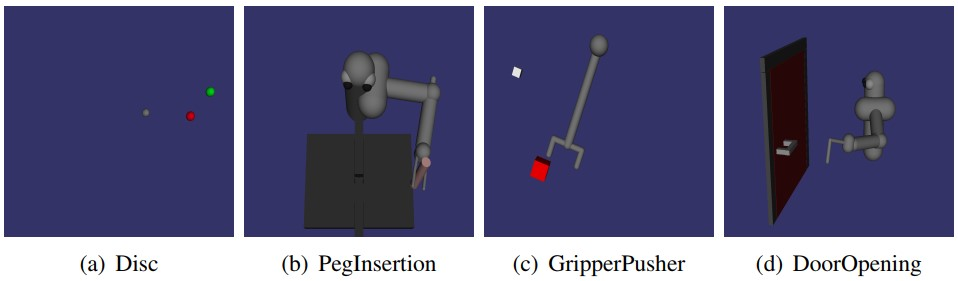
\includegraphics[width=\textwidth]{Figures/images/dealio/dealio_performed_task.jpg}
        \caption{Control Tasks solved in~\cite{torabi2021dealio}}
        \label{fig:dealio_task}
    \end{subfigure}
    \vfill
    \begin{subfigure}[b]{0.8\textwidth}
        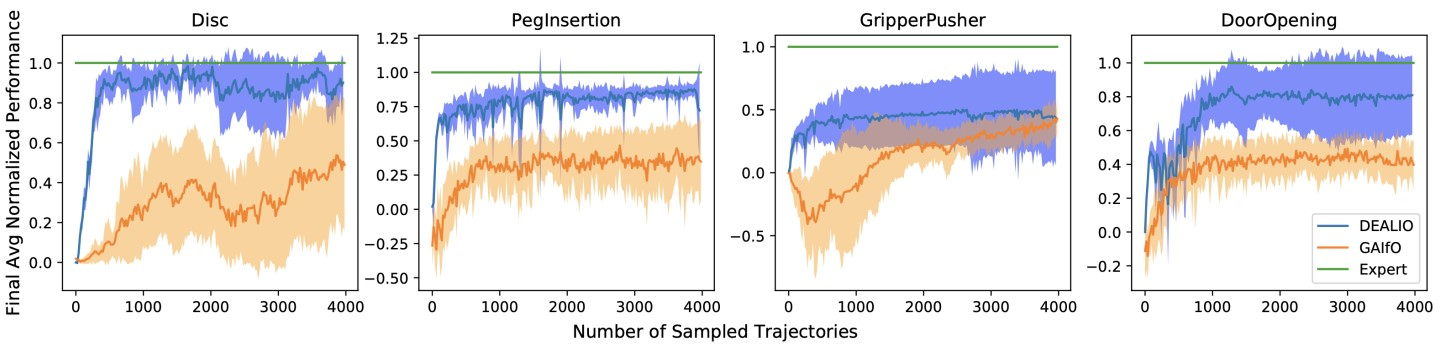
\includegraphics[width=\textwidth]{Figures/images/dealio/dealio_performance.jpg}
        \caption{Performance of DEALIO~\cite{torabi2021dealio} compared against GAIfO~\cite{torabi2018gaifo}, with respect to the number of trajectories sampled during the learning process.}
        \label{fig:dealio_performance}
    \end{subfigure}
    \caption{DEAILO: (\ref{fig:dealio_task}) Control Tasks, (\ref{fig:dealio_performance}) Performance Level}
    \label{fig:dealio}
\end{figure}


Generally, LfO methods have demonstrated interesting features, such as generating a policy from state-based information alone. This supports the hypothesis that the primary source of information for task learning is the sequence of state transitions. Extrapolating the valuable information to perform actions that induce the desired behavior may not be trivial, especially if the state space is represented by images of a human operator. This complexity leads to the design of architectures composed of different stages, which not only increase the complexity of the system itself but also the amount and diversity of data required for their training. Furthermore, many methods of interest have been tested in simulated or relatively simple scenarios, still leaving open whether these methods can be used in real-world complex robotic manipulation tasks.






